\chapter{Resultados}

Este capítulo apresenta os resultados obtidos com a aplicação desenvolvida e uma discussão acerca destes. A análise dos resultados será feita através da comparação dos dois descritores implementados. Antes de apresentar os resultados com imagens provenientes de uma busca, serão apresentados resultados do algoritmo em uma página de testes. As páginas de testes foram usadas como guias de ajustes e validação visual do algoritmo proposto.

A Tabela \ref{paginaTeste} apresenta as imagens presentes em uma página de teste. Apesar de todas estas imagens serem diferentes, as características que elas carregam são semelhantes entre algumas. As imagens da linha um são de tomates apresentados em diferentes ângulos em uma imagem de fundo próximo ao branco. Semelhantemente, a linha dois apresenta imagens de balões com fundo azul não necessariamente na mesma tonalidade. 

\begin{table}[h]
    \begin{center}
      \caption{Imagens de página de teste.}
\begin{tabular}{ |>{\centering\arraybackslash}m{5cm} | >{\centering\arraybackslash}m{5cm} | >{\centering\arraybackslash}m{5cm} | } 
\hline
   \begin{subfigure}[b]{5cm}
   \centering
   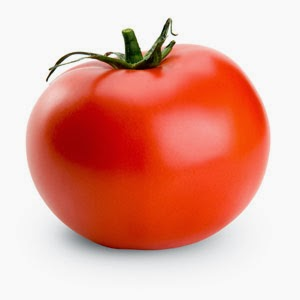
\includegraphics[width=5cm,height=4cm,keepaspectratio,trim=0 0 0 -5]{images/paginaTeste/tomate1.jpg}
   \caption*{1}
  \end{subfigure}
   &
    \begin{subfigure}[b]{5cm}
  \centering
   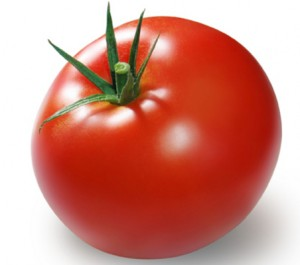
\includegraphics[width=5cm,height=4cm,keepaspectratio,trim=0 0 0 -5]{images/paginaTeste/tomate2.jpg}
   \caption*{2}
  \end{subfigure}
   & 
    \begin{subfigure}[b]{5cm}
  \centering
   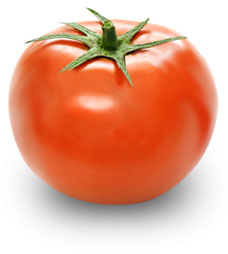
\includegraphics[width=5cm,height=4cm,keepaspectratio,trim=0 0 0 -5]{images/paginaTeste/tomate3.jpg}
   \caption*{3}
  \end{subfigure} \\ 
 \hline
   \begin{subfigure}[b]{5cm}
  \centering
   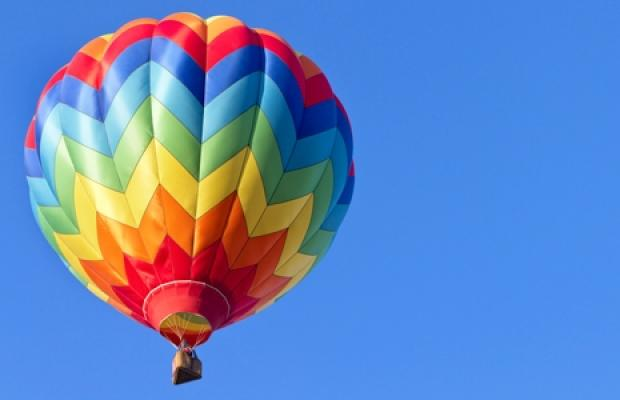
\includegraphics[width=5cm,height=4cm,keepaspectratio,trim=0 0 0 -5]{images/paginaTeste/balao1.jpg}
   \caption*{4}
  \end{subfigure}
   &
   \begin{subfigure}[b]{5cm}
  \centering
   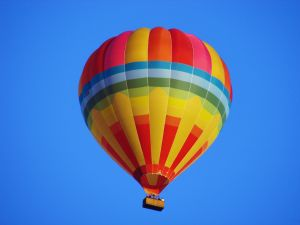
\includegraphics[width=5cm,height=4cm,keepaspectratio,trim=0 0 0 -5]{images/paginaTeste/balao2.jpg}
	\caption*{5}
   \end{subfigure}
   & 
   \begin{subfigure}[b]{5cm}
  \centering
    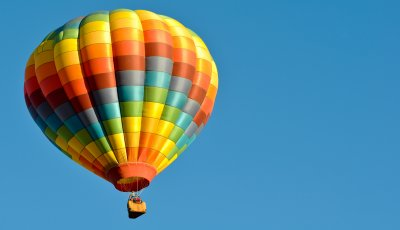
\includegraphics[width=5cm,height=4cm,keepaspectratio,trim=0 0 0 -5]{images/paginaTeste/balao3.jpg}
    \caption*{6}
  \end{subfigure} \\ 
 
 \hline
\end{tabular}
\label{paginaTeste}
\legend{\textbf{Fonte:} \citeonline{google0, google1}.}
\end{center}
\end{table}

A matriz de distâncias entre as imagens calculada através dos autovetores dominantes é apresentada na Tabela \ref{matrizDistanciaAutoVetores} e a calculada através dos histogramas é apresentada na Tabela \ref{matrizDistanciaHistogramas}. As células destacadas indicam os dois menores valores, ou seja as duas imagens mais próximas.

\begin{sidewaystable}[pht!]

\centering
    \caption{Matriz de distâncias - Autovetores Dominantes.}
\begin{tabular}{|l|l|l|l|l|l|l|}
        \hline
         & 1 & 2  & 3 & 4 & 5 & 6   \\ \hline
        1   &  0 & \cellcolor{blue!25}0.7903890183496494 & \cellcolor{blue!25}1.267739792773765 & 1.5707963267948966 &  1.5707960225553694 & 1.5707963267027802\\ 
        \hline
        2   &  \cellcolor{blue!25}0.7903890183496494& 0& \cellcolor{blue!25}1.1557908824986878& 1.5707963267948966 &  1.5707962171666512 & 1.5707963266958864\\
        \hline 
        3   &  \cellcolor{blue!25}1.267739792773765 & \cellcolor{blue!25}1.1557908824986878 & 0 & 1.5707963267948966 &  1.5632618141959285 & 1.5707963267041545\\ 
        \hline
        4   &  1.5707963267948966 & 1.5707963267948966 & 1.5707963267948966 & 0 &  \cellcolor{blue!25}1.5707962924625574 & \cellcolor{blue!25}1.5707804758766788\\ 
        \hline
        5   &  1.5707960225553694 & 1.5707962171666512 & 1.5632618141959285 & \cellcolor{blue!25}1.5707962924625574 &  0 & \cellcolor{blue!25}1.5707679774026786\\ 
        \hline
        6   &  1.5707963267027802 & 1.5707963266958864 & 1.5707963267041545 & \cellcolor{blue!25}1.5707804758766788 &  \cellcolor{blue!25}1.5707679774026786 & 0\\ 
        \hline
    \end{tabular}
\label{matrizDistanciaAutoVetores}
    \legend{\textbf{Fonte}: Autoria Própria}

\centering
    \caption{Matriz de distâncias - Histogramas.}
\begin{tabular}{|l|l|l|l|l|l|l|}
        \hline
         & 1 & 2  & 3 & 4 & 5 & 6   \\ \hline
        1   &  0 & \cellcolor{blue!25}0.5756075471698113 & \cellcolor{blue!25}0.5971680480729381 & 0.6794026881720429 &  0.6567888888888888 & 0.7045434782608694\\ 
        \hline
        2   &  \cellcolor{blue!25}0.5756075471698113 & 0& \cellcolor{blue!25}0.42156721584082& 0.6947065074051536 &  0.7187795946890287 & 0.7458547990155866\\ 
        \hline
        3   &  \cellcolor{blue!25}0.5971680480729381 & \cellcolor{blue!25}0.42156721584082 & 0 & 0.6477030282876355 &  0.588672665039677 & 0.6363063718865803\\ 
        \hline
        4   &  0.6794026881720429 & 0.6947065074051536 & 0.6477030282876355 & 0 &  \cellcolor{blue!25}0.4964178912783750 & \cellcolor{blue!25}0.2739817671809256\\
        \hline 
        5   &  0.6567888888888888 & 0.7187795946890287 & 0.588672665039677 & \cellcolor{blue!25}0.4964178912783750 &  0 & \cellcolor{blue!25}0.3671427536231884\\ 
        \hline
        6   &  0.7045434782608694 & 0.7458547990155866 & 0.6363063718865803 & \cellcolor{blue!25}0.2739817671809256 &  \cellcolor{blue!25}0.3671427536231884 & 0\\ 
        \hline
    \end{tabular}
\label{matrizDistanciaHistogramas}
    \legend{\textbf{Fonte}: Autoria Própria}

\end{sidewaystable}

\pagebreak

Como esperado, o algoritmo de agrupamento por nuvens dinâmicas alocou todas as imagens da linha um (tomates) em um grupo e consequentemente as imagens da linha dois (balões) foram alocadas em um grupo distinto.

A seguir são apresentados os resultados da aplicação e da busca pelas palavras chaves, casa, lentilha e gato. As Tabelas \ref{chaves}, \ref{casa}, \ref{lentilha} e \ref{gato} apresentam as imagens na ordem inicial disposta na página do \emph{Google}. As outras tabelas apresentam os resultados obtidos através da extensão e dispõem as imagens de acordo com as alocações de forma que cada agrupamento é identificado por uma cor de fundo. Cada imagem é identificada por um número e os protótipos de cada grupo são identificados pelo número de identificação entre colchetes.

A Tabela \ref{chavesAutoVetor} apresenta o conjunto de imagens da Tabela \ref{chaves} organizado em três grupos. É possível observar que neste conjunto existem imagens similares como 1, 10, 13, 11, 21 que foram alocadas no mesmo grupo. De maneira semelhante, as imagens 0 e 8 foram alocadas no mesmo grupo. Entretanto, também é possível observar que as imagens 25 e 32 foram alocadas em grupos diferentes sendo que elas são visualmente parecidas, apesar de uma ser colorida e a outra não. Isto pode acontecer devido a diferenças como contraste por exemplo.

O resultado para o conjunto de imagens da Tabela \ref{chaves} em três grupos usando os histogramas como descritores está disposto na Tabela \ref{chavesHistograma}. Com o uso de histogramas como descritores, parecem mais heterogêneos se comparados aos grupos da Tabela \ref{chavesAutoVetor}. Desta forma, para este conjunto de dados, o uso dos autovetores dominantes parece mais adequado.

As imagens da Tabela \ref{lentilha} apresentam o conjunto de imagens obtido na pesquisa pela palavra lentilha. Este conjunto foi organizado em quatro grupos. Neste conjunto é possível observar várias imagens com regiões das cores marrom, branca e bege. Os resultados usando os autovetores dominantes são apresentados na Tabela \ref{lentilhaAutoVetor} e os resultados usando os histogramas estão na Tabela \ref{histogramas}.

O uso dos histogramas pareceu mais adequado para o conjunto de dados da Tabela \ref{lentilha} uma vez que a Tabela \ref{lentilhaHistograma} apresenta imagens melhores distribuídas de acordo com os aspectos visuais. No grupo um é possível ver imagens com predominância do branco e com cores concentradas no centro das imagens enquanto que o grupo dois apresenta imagens com cores mais distribuídas em meio ao branco assim como o grupo quatro. O grupo três concentra as imagens com regiões de cor marrom representadas pela imagem 26 que é o protótipo do grupo.

As imagens da Tabela \ref{casa} foram divididas em cinco grupos. Neste conjunto de dados é possível observar algumas imagens com características visualmente semelhantes, como as imagens 0, 2, 5, 6, 10, 11, 16, 30, 31, 32 que possuem fundo branco. Além dessas imagens é possível observar que apesar de algumas imagens não possuírem fundo branco, têm o branco predominando.

A Tabela \ref{casaAutoVetor} mostra os resultados da aplicação ao usar os autovetores dominantes como descritores. É possível observar que o primeiro grupo é homogêneo, mas poderia incluir outras imagens com as mesmas características como 16, 6, 2, 5, 10 e 30. Os elementos do segundo grupo parecem similares ao possuírem regiões verdes e regiões escuras. O terceiro grupo apresenta o elemento 28 que visualmente se encaixaria na característica tida como dominante do grupo dois. Apesar disso, as outras imagens do grupo se assemelham assim como as imagens dos próximos grupos.

A Tabela \ref{casaHistograma} apresenta os resultados usando os histogramas como descritores e assim como na Tabela \ref{casaAutoVetor}, algumas imagens com características predominantes brancas foram agrupadas em grupos diferentes. Entretanto isso não significa que os grupos estão heterogêneos como em alguns grupos dos resultados do outro descritor, mas que os grupos 1, 3 e 5 são semelhantes. Os grupos dois e quatro são homogêneos, o dois ao apresentar claramente imagens predominantemente com regiões escuras não encontradas em outras imagens do conjunto.

O conjunto de imagens da Tabela \ref{gato} apresenta o conjunto de imagens obtidas através da busca por gato que foi dividido em seis grupos. Para este conjunto, os resultados usando os autovetores dominantes e histogramas estão dispostos na Tabela \ref{gatoAutoVetor} e Tabela \ref{gatoHistograma} respectivamente.

Para o conjunto de dados da Tabela \ref{gato} os resultados com os autovetores dominantes se apresentaram mais satisfatórios se comparados aos resultados do outro descritor. O fato é que os resultados da Tabela \ref{gatoHistograma} não se apresentam criteriosos nas divisões apresentadas enquanto que os resultados da Tabela \ref{gatoAutoVetor} estão melhores distribuídos. 

O grupo um da Tabela \ref{gatoAutoVetor} apresenta imagens com aspectos mais neutros se comparadas as outras imagens do mesmo conjunto, mas é possível observar que o restante dos grupos apresenta resultados mais semelhantes. O grupo dois contém imagens com tons de cinza com baixo contraste, em contrapartida o grupo cinco dispõe de imagens com mais contraste. O grupo quatro destes resultados se destaca ao ter todas as imagens com gatos alaranjados. Além do grupo quatro, o grupo seis também se mostra homogêneo ao dispor de imagens de gatos ao centro com fundo predominantemente branco.

\newpage
\begin{table}[h]
    \begin{center}
      \caption{Imagens de página de pesquisa - Chaves.}
\begin{tabular}{ |>{\centering\arraybackslash}m{4.9cm} | >{\centering\arraybackslash}m{4.9cm} | >{\centering\arraybackslash}m{4.9cm} | } 
\hline
	\grbox{
   \begin{subfigure}[b]{5cm}
   \centering
   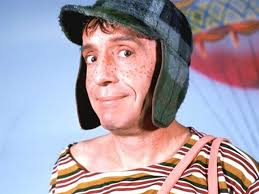
\includegraphics[width=5cm,height=2cm,keepaspectratio,trim=0 0 0 -5]{images/chaves/0.jpeg}
  \end{subfigure}}{0}
   &
   \grbox{
    \begin{subfigure}[b]{5cm}
  \centering
   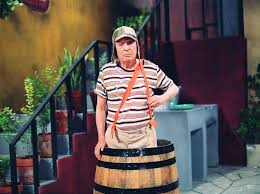
\includegraphics[width=5cm,height=2cm,keepaspectratio,trim=0 0 0 -5]{images/chaves/1.jpeg}
  \end{subfigure}}{1}
   & 
   \grbox{
    \begin{subfigure}[b]{5cm}
  \centering
   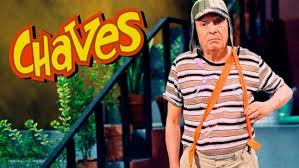
\includegraphics[width=5cm,height=2cm,keepaspectratio,trim=0 0 0 -5]{images/chaves/2.jpeg}
  \end{subfigure}}{2} \\ 
 \hline
 \grbox{
   \begin{subfigure}[b]{5cm}
  \centering
   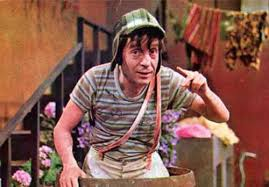
\includegraphics[width=5cm,height=2cm,keepaspectratio,trim=0 0 0 -5]{images/chaves/3.jpeg}
  \end{subfigure}}{3}
   &
   \grbox{
   \begin{subfigure}[b]{5cm}
  \centering
   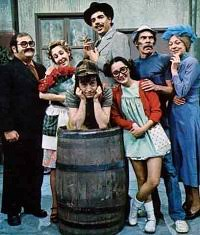
\includegraphics[width=5cm,height=2cm,keepaspectratio,trim=0 0 0 -5]{images/chaves/4.jpeg}
   \end{subfigure}}{4}
   & 
   \grbox{
   \begin{subfigure}[b]{5cm}
  \centering
    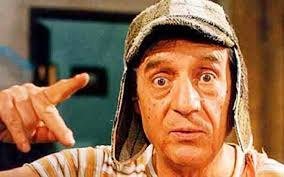
\includegraphics[width=5cm,height=2cm,keepaspectratio,trim=0 0 0 -5]{images/chaves/5.jpeg}
  \end{subfigure}}{5} \\ 
   \hline
   \grbox{
   \begin{subfigure}[b]{5cm}
  \centering
   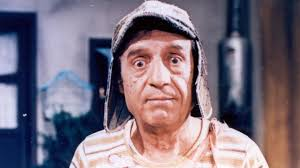
\includegraphics[width=5cm,height=2cm,keepaspectratio,trim=0 0 0 -5]{images/chaves/6.jpeg}
   \end{subfigure}}{6}
   &
   \grbox{
   \begin{subfigure}[b]{5cm}
  \centering
   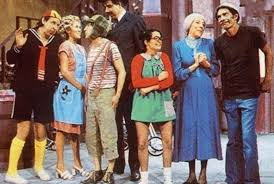
\includegraphics[width=5cm,height=2cm,keepaspectratio,trim=0 0 0 -5]{images/chaves/7.jpeg}
   \end{subfigure}}{7}
   & 
   \grbox{
   \begin{subfigure}[b]{5cm}
  \centering
    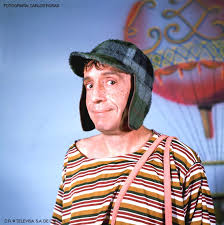
\includegraphics[width=5cm,height=2cm,keepaspectratio,trim=0 0 0 -5]{images/chaves/8.jpeg}
  \end{subfigure}}{8} \\ 
   \hline
   \grbox{
   \begin{subfigure}[b]{5cm}
  \centering
   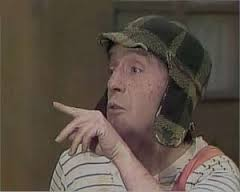
\includegraphics[width=5cm,height=2cm,keepaspectratio,trim=0 0 0 -5]{images/chaves/9.jpeg}
  \end{subfigure}}{9}
   &
   \grbox{
   \begin{subfigure}[b]{5cm}
  \centering
   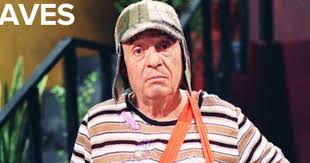
\includegraphics[width=5cm,height=2cm,keepaspectratio,trim=0 0 0 -5]{images/chaves/10.jpeg}
   \end{subfigure}}{10}
   & 
   \grbox{
   \begin{subfigure}[b]{5cm}
  \centering
    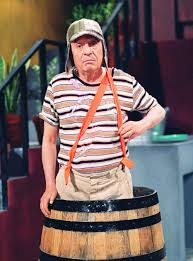
\includegraphics[width=5cm,height=2cm,keepaspectratio,trim=0 0 0 -5]{images/chaves/11.jpeg}
  \end{subfigure}}{11} \\ 
   \hline
   \grbox{
   \begin{subfigure}[b]{5cm}
  \centering
   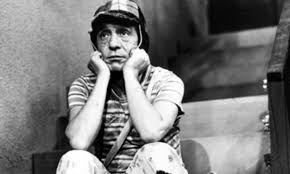
\includegraphics[width=5cm,height=2cm,keepaspectratio,trim=0 0 0 -5]{images/chaves/12.jpeg}
  \end{subfigure}}{12}
   &
   \grbox{
   \begin{subfigure}[b]{5cm}
  \centering
   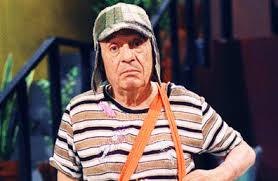
\includegraphics[width=5cm,height=2cm,keepaspectratio,trim=0 0 0 -5]{images/chaves/13.jpeg}
   \end{subfigure}}{13}
   & 
   \grbox{
   \begin{subfigure}[b]{5cm}
  \centering
    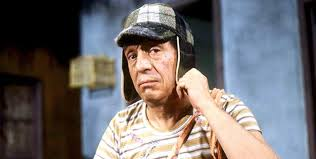
\includegraphics[width=5cm,height=2cm,keepaspectratio,trim=0 0 0 -5]{images/chaves/14.jpeg}
  \end{subfigure}}{14} \\ 
   \hline
   \grbox{
   \begin{subfigure}[b]{5cm}
  \centering
   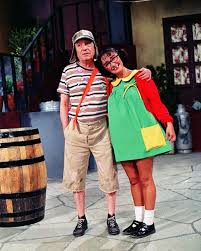
\includegraphics[width=5cm,height=2cm,keepaspectratio,trim=0 0 0 -5]{images/chaves/15.jpeg}
  \end{subfigure}}{15}
   &
   \grbox{
   \begin{subfigure}[b]{5cm}
  \centering
   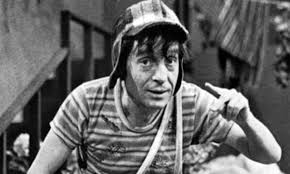
\includegraphics[width=5cm,height=2cm,keepaspectratio,trim=0 0 0 -5]{images/chaves/16.jpeg}
   \end{subfigure}}{16}
   & 
   \grbox{
   \begin{subfigure}[b]{5cm}
  \centering
    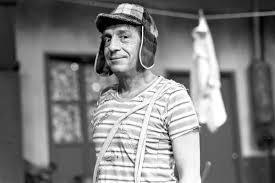
\includegraphics[width=5cm,height=2cm,keepaspectratio,trim=0 0 0 -5]{images/chaves/17.jpeg}
  \end{subfigure}}{17} \\ 
   \hline
   \grbox{
   \begin{subfigure}[b]{5cm}
  \centering
   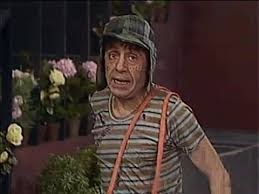
\includegraphics[width=5cm,height=2cm,keepaspectratio,trim=0 0 0 -5]{images/chaves/18.jpeg}
  \end{subfigure}}{18}
   &
   \grbox{
   \begin{subfigure}[b]{5cm}
  \centering
   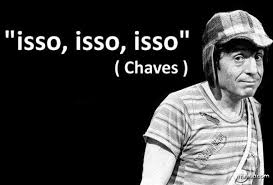
\includegraphics[width=5cm,height=2cm,keepaspectratio,trim=0 0 0 -5]{images/chaves/19.jpeg}
   \end{subfigure}}{19}
   & 
   \grbox{
   \begin{subfigure}[b]{5cm}
  \centering
    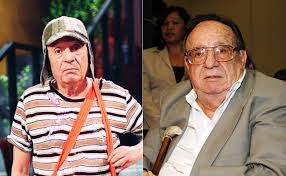
\includegraphics[width=5cm,height=2cm,keepaspectratio,trim=0 0 0 -5]{images/chaves/20.jpeg}
  \end{subfigure}}{20} \\ 
   \hline
   \grbox{
   \begin{subfigure}[b]{5cm}
  \centering
   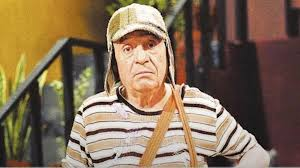
\includegraphics[width=5cm,height=2cm,keepaspectratio,trim=0 0 0 -5]{images/chaves/21.jpeg}
  \end{subfigure}}{21}
   &
   \grbox{
   \begin{subfigure}[b]{5cm}
  \centering
   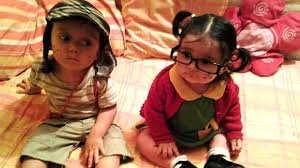
\includegraphics[width=5cm,height=2cm,keepaspectratio,trim=0 0 0 -5]{images/chaves/22.jpeg}
   \end{subfigure}}{22}
   & 
   \grbox{
   \begin{subfigure}[b]{5cm}
  \centering
    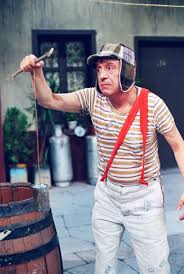
\includegraphics[width=5cm,height=2cm,keepaspectratio,trim=0 0 0 -5]{images/chaves/23.jpeg}
  \end{subfigure}}{23} \\
 \hline
 \grbox{
 \begin{subfigure}[b]{5cm}
  \centering
   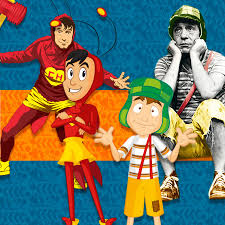
\includegraphics[width=5cm,height=2cm,keepaspectratio,trim=0 0 0 -5]{images/chaves/24.jpeg}
  \end{subfigure}}{24}
   &
   \grbox{
   \begin{subfigure}[b]{5cm}
  \centering
   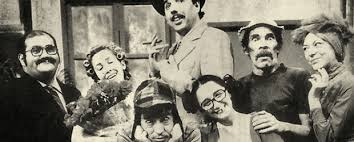
\includegraphics[width=4.2cm,height=2cm,keepaspectratio,trim=0 0 0 -5]{images/chaves/25.jpeg}
   \end{subfigure}}{25}
   & 
   \grbox{
   \begin{subfigure}[b]{5cm}
  \centering
    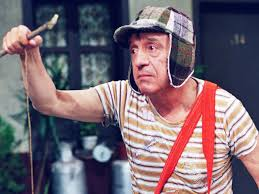
\includegraphics[width=5cm,height=2cm,keepaspectratio,trim=0 0 0 -5]{images/chaves/26.jpeg}
  \end{subfigure}}{26} \\
 \hline
 \grbox{
 \begin{subfigure}[b]{5cm}
  \centering
   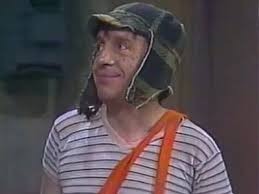
\includegraphics[width=5cm,height=2cm,keepaspectratio,trim=0 0 0 -5]{images/chaves/27.jpeg}
  \end{subfigure}}{27}
   &
   \grbox{
   \begin{subfigure}[b]{5cm}
  \centering
   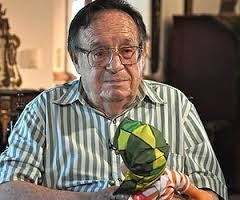
\includegraphics[width=5cm,height=2cm,keepaspectratio,trim=0 0 0 -5]{images/chaves/28.jpeg}
   \end{subfigure}}{28}
   & 
   \grbox{
   \begin{subfigure}[b]{5cm}
  \centering
    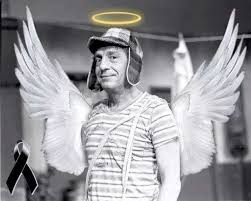
\includegraphics[width=5cm,height=2cm,keepaspectratio,trim=0 0 0 -5]{images/chaves/29.jpeg}
  \end{subfigure}}{29} \\
 \hline
 \grbox{
 \begin{subfigure}[b]{5cm}
  \centering
   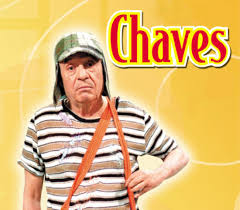
\includegraphics[width=5cm,height=2cm,keepaspectratio,trim=0 0 0 -5]{images/chaves/30.jpeg}
  \end{subfigure}}{30}
   &
   \grbox{
   \begin{subfigure}[b]{5cm}
  \centering
   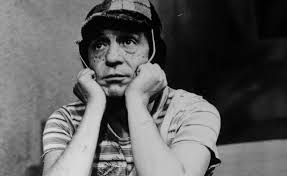
\includegraphics[width=5cm,height=2cm,keepaspectratio,trim=0 0 0 -5]{images/chaves/31.jpeg}
  \end{subfigure}}{31}
   &
   \grbox{
   \begin{subfigure}[b]{5cm}
  \centering
   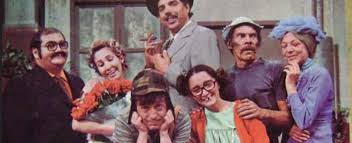
\includegraphics[width=4.2cm,height=2cm,keepaspectratio,trim=0 0 0 -5]{images/chaves/32.jpeg}
  \end{subfigure}}{32}  \\
 \hline
\end{tabular}
\label{chaves}
\legend{\textbf{Fonte:} \citeonline{google2}.}
\end{center}
\end{table}

\newpage

\colorlet{cluster1}{blue!25}
\colorlet{cluster2}{gray}
\definecolor{cluster3}{rgb}{0.88,1,1}
\begin{table}[h]
    \begin{center}
      \caption{Autovetor - Resultado do conjunto chaves em 3 grupos.}
\begin{tabular}{ |>{\centering\arraybackslash}m{4.9cm} | >{\centering\arraybackslash}m{4.9cm} | >{\centering\arraybackslash}m{4.9cm} | } 
	\hline
	\cellcolor{cluster1}
	\grbox{
   \begin{subfigure}[b]{5cm}
   \centering
   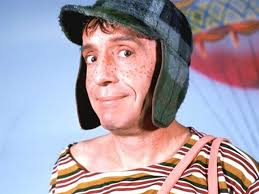
\includegraphics[width=5cm,height=2cm,keepaspectratio,trim=0 0 0 -5]{images/chaves/0.jpeg}
  \end{subfigure}}{0}
   &
   \cellcolor{cluster1}
   \grbox{
    \begin{subfigure}[b]{5cm}
  \centering
   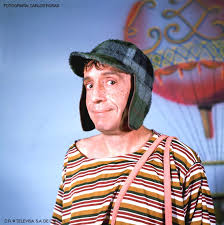
\includegraphics[width=5cm,height=2cm,keepaspectratio,trim=0 0 0 -5]{images/chaves/8.jpeg}
  \end{subfigure}}{8}
   & 
   \cellcolor{cluster1}
   \grbox{
    \begin{subfigure}[b]{5cm}
  \centering
   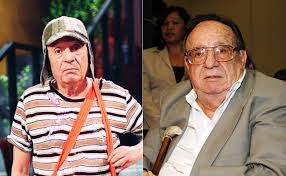
\includegraphics[width=5cm,height=2cm,keepaspectratio,trim=0 0 0 -5]{images/chaves/20.jpeg}
  \end{subfigure}}{20} \\ 
 
 \cellcolor{cluster1}
 \grbox{
   \begin{subfigure}[b]{5cm}
  \centering
   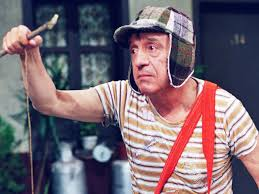
\includegraphics[width=5cm,height=2cm,keepaspectratio,trim=0 0 0 -5]{images/chaves/26.jpeg}
  \end{subfigure}}{26}
   &
   \cellcolor{cluster1}
   \grbox{
   \begin{subfigure}[b]{5cm}
  \centering
   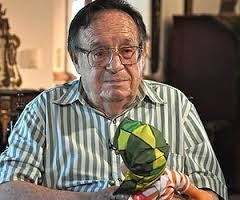
\includegraphics[width=5cm,height=2cm,keepaspectratio,trim=0 0 0 -5]{images/chaves/28.jpeg}
   \end{subfigure}}{28}
   & 
   \cellcolor{cluster1}
   \grbox{
   \begin{subfigure}[b]{5cm}
  \centering
    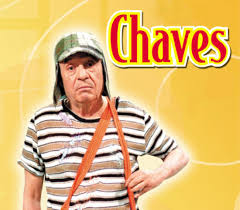
\includegraphics[width=5cm,height=2cm,keepaspectratio,trim=0 0 0 -5]{images/chaves/30.jpeg}
  \end{subfigure}}{30} \\ 
   \cellcolor{cluster1}
   \grbox{
   \begin{subfigure}[b]{5cm}
  \centering
   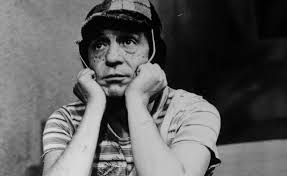
\includegraphics[width=5cm,height=2cm,keepaspectratio,trim=0 0 0 -5]{images/chaves/31.jpeg}
  \end{subfigure}}{\underline{31}}
   &
   \cellcolor{cluster2}
   \grbox{
   \begin{subfigure}[b]{5cm}
  \centering
   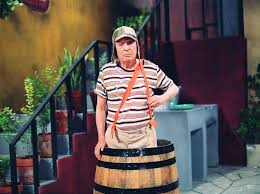
\includegraphics[width=5cm,height=2cm,keepaspectratio,trim=0 0 0 -5]{images/chaves/1.jpeg}
   \end{subfigure}}{1}
   & 
   \cellcolor{cluster2}
   \grbox{
   \begin{subfigure}[b]{5cm}
  \centering
    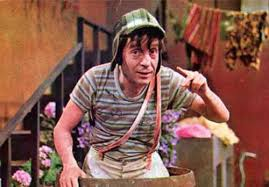
\includegraphics[width=5cm,height=2cm,keepaspectratio,trim=0 0 0 -5]{images/chaves/3.jpeg}
  \end{subfigure}}{3} \\ 
   
   \cellcolor{cluster2}
   \grbox{
   \begin{subfigure}[b]{5cm}
  \centering
   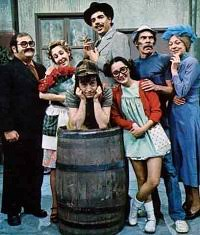
\includegraphics[width=5cm,height=2cm,keepaspectratio,trim=0 0 0 -5]{images/chaves/4.jpeg}
  \end{subfigure}}{4}
   &
   \cellcolor{cluster2}
   \grbox{
   \begin{subfigure}[b]{5cm}
  \centering
   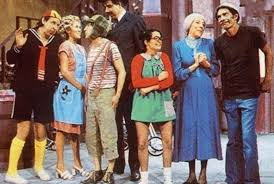
\includegraphics[width=5cm,height=2cm,keepaspectratio,trim=0 0 0 -5]{images/chaves/7.jpeg}
   \end{subfigure}}{7}
   & 
   \cellcolor{cluster2}
   \grbox{
   \begin{subfigure}[b]{5cm}
  \centering
    \includegraphics[width=5cm,height=2cm,keepaspectratio,trim=0 0 0 -5]{images/chaves/9.jpeg}
  \end{subfigure}}{9} \\ 
   
   \cellcolor{cluster2}
   \grbox{
   \begin{subfigure}[b]{5cm}
  \centering
   \includegraphics[width=5cm,height=2cm,keepaspectratio,trim=0 0 0 -5]{images/chaves/10.jpeg}
  \end{subfigure}}{10}
   &
   \cellcolor{cluster2}
   \grbox{
   \begin{subfigure}[b]{5cm}
  \centering
   \includegraphics[width=5cm,height=2cm,keepaspectratio,trim=0 0 0 -5]{images/chaves/11.jpeg}
   \end{subfigure}}{11}
   & 
   \cellcolor{cluster2}
   \grbox{
   \begin{subfigure}[b]{5cm}
  \centering
    \includegraphics[width=5cm,height=2cm,keepaspectratio,trim=0 0 0 -5]{images/chaves/12.jpeg}
  \end{subfigure}}{12} \\ 
   
   \cellcolor{cluster2}
   \grbox{
   \begin{subfigure}[b]{5cm}
  \centering
   \includegraphics[width=5cm,height=2cm,keepaspectratio,trim=0 0 0 -5]{images/chaves/13.jpeg}
  \end{subfigure}}{13}
   &
   \cellcolor{cluster2}
   \grbox{
   \begin{subfigure}[b]{5cm}
  \centering
   \includegraphics[width=5cm,height=2cm,keepaspectratio,trim=0 0 0 -5]{images/chaves/15.jpeg}
   \end{subfigure}}{15}
   & 
   \cellcolor{cluster2}
   \grbox{
   \begin{subfigure}[b]{5cm}
  \centering
    \includegraphics[width=5cm,height=2cm,keepaspectratio,trim=0 0 0 -5]{images/chaves/18.jpeg}
  \end{subfigure}}{\underline{18}} \\ 
   
   \cellcolor{cluster2}
   \grbox{
   \begin{subfigure}[b]{5cm}
  \centering
   \includegraphics[width=5cm,height=2cm,keepaspectratio,trim=0 0 0 -5]{images/chaves/21.jpeg}
  \end{subfigure}}{21}
   &
   \cellcolor{cluster2}
   \grbox{
   \begin{subfigure}[b]{5cm}
  \centering
   \includegraphics[width=5cm,height=2cm,keepaspectratio,trim=0 0 0 -5]{images/chaves/22.jpeg}
   \end{subfigure}}{22}
   & 
   \cellcolor{cluster2}
   \grbox{
   \begin{subfigure}[b]{5cm}
  \centering
    \includegraphics[width=5cm,height=2cm,keepaspectratio,trim=0 0 0 -5]{images/chaves/23.jpeg}
  \end{subfigure}}{23} \\ 
   
   \cellcolor{cluster2}
   \grbox{
   \begin{subfigure}[b]{5cm}
  \centering
   \includegraphics[width=5cm,height=2cm,keepaspectratio,trim=0 0 0 -5]{images/chaves/24.jpeg}
  \end{subfigure}}{24}
   &
   \cellcolor{cluster2}
   \grbox{
   \begin{subfigure}[b]{5cm}
  \centering
   \includegraphics[width=4.2cm,height=2cm,keepaspectratio,trim=0 0 0 -5]{images/chaves/25.jpeg}
   \end{subfigure}}{25}
   & 
   \cellcolor{cluster2}
   \grbox{
   \begin{subfigure}[b]{5cm}
  \centering
    \includegraphics[width=5cm,height=2cm,keepaspectratio,trim=0 0 0 -5]{images/chaves/27.jpeg}
  \end{subfigure}}{28} \\
 
 \cellcolor{cluster2}
 \grbox{
 \begin{subfigure}[b]{5cm}
  \centering
   \includegraphics[width=5cm,height=2cm,keepaspectratio,trim=0 0 0 -5]{images/chaves/29.jpeg}
  \end{subfigure}}{29}
   &
   \cellcolor{cluster3}
   \grbox{
   \begin{subfigure}[b]{5cm}
  \centering
   \includegraphics[width=5cm,height=2cm,keepaspectratio,trim=0 0 0 -5]{images/chaves/2.jpeg}
   \end{subfigure}}{2}
   & 
   \cellcolor{cluster3}
   \grbox{
   \begin{subfigure}[b]{5cm}
  \centering
    \includegraphics[width=5cm,height=2cm,keepaspectratio,trim=0 0 0 -5]{images/chaves/5.jpeg}
  \end{subfigure}}{5} \\
  \cellcolor{cluster3}
  \grbox{
 \begin{subfigure}[b]{5cm}
  \centering
   \includegraphics[width=5cm,height=2cm,keepaspectratio,trim=0 0 0 -5]{images/chaves/6.jpeg}
  \end{subfigure}}{6}
   &
   \cellcolor{cluster3}
   \grbox{
   \begin{subfigure}[b]{5cm}
  \centering
   \includegraphics[width=5cm,height=2cm,keepaspectratio,trim=0 0 0 -5]{images/chaves/14.jpeg}
   \end{subfigure}}{14}
   & 
   \cellcolor{cluster3}
   \grbox{
   \begin{subfigure}[b]{5cm}
  \centering
    \includegraphics[width=5cm,height=2cm,keepaspectratio,trim=0 0 0 -5]{images/chaves/16.jpeg}
  \end{subfigure}}{16} \\
 \cellcolor{cluster3}
 \grbox{
 \begin{subfigure}[b]{5cm}
  \centering
   \includegraphics[width=5cm,height=2cm,keepaspectratio,trim=0 0 0 -5]{images/chaves/17.jpeg}
  \end{subfigure}}{17}
   &
   \cellcolor{cluster3}
   \grbox{
   \begin{subfigure}[b]{5cm}
  \centering
   \includegraphics[width=5cm,height=2cm,keepaspectratio,trim=0 0 0 -5]{images/chaves/19.jpeg}
  \end{subfigure}}{\underline{19}}
   &
   \cellcolor{cluster3}
   \grbox{
   \begin{subfigure}[b]{5cm}
  \centering
   \includegraphics[width=4.2cm,height=2cm,keepaspectratio,trim=0 0 0 -5]{images/chaves/32.jpeg}
  \end{subfigure}}{32}  \\
  \hline
\end{tabular}
\label{chavesAutoVetor}
\legend{\textbf{Fonte:} \citeonline{google2}.}
\end{center}
\end{table}

\newpage

\colorlet{cluster1}{blue!25}
\colorlet{cluster3}{gray}
\definecolor{cluster3}{rgb}{0.88,1,1}
\begin{table}[h]
    \begin{center}
      \caption{Histograma - Resultado do conjunto chaves em 3 grupos.}
\begin{tabular}{ |>{\centering\arraybackslash}m{4.9cm} | >{\centering\arraybackslash}m{4.9cm} | >{\centering\arraybackslash}m{4.9cm} | } 
	\hline
	\cellcolor{cluster1}
   \grbox{
   \begin{subfigure}[b]{5cm}
   \centering
   \includegraphics[width=5cm,height=2cm,keepaspectratio,trim=0 0 0 -5]{images/chaves/0.jpeg} 
	\end{subfigure}}{0}
   &
   \cellcolor{cluster1}
    \grbox{
   \begin{subfigure}[b]{5cm}
  \centering
   \includegraphics[width=5cm,height=2cm,keepaspectratio,trim=0 0 0 -5]{images/chaves/29.jpeg} 
	\end{subfigure}}{\underline{29}}
   & 
   \cellcolor{cluster1}
    \grbox{
   \begin{subfigure}[b]{5cm}
  \centering
   \includegraphics[width=5cm,height=2cm,keepaspectratio,trim=0 0 0 -5]{images/chaves/30.jpeg} 
	\end{subfigure}}{30}
 \\ 
 \cellcolor{cluster2}
   \grbox{
   \begin{subfigure}[b]{5cm}
  \centering
   \includegraphics[width=5cm,height=2cm,keepaspectratio,trim=0 0 0 -5]{images/chaves/8.jpeg} 
	\end{subfigure}}{\underline{8}}
   &
   \cellcolor{cluster2}
   \grbox{
   \begin{subfigure}[b]{5cm}
  \centering
   \includegraphics[width=5cm,height=2cm,keepaspectratio,trim=0 0 0 -5]{images/chaves/31.jpeg} 
	\end{subfigure}}{31}
   & 
   \cellcolor{cluster3}
   \grbox{
   \begin{subfigure}[b]{5cm}
  \centering
    \includegraphics[width=5cm,height=2cm,keepaspectratio,trim=0 0 0 -5]{images/chaves/2.jpeg} 
	\end{subfigure}}{2}
 \\ 
   \cellcolor{cluster3}
   \grbox{
   \begin{subfigure}[b]{5cm}
  \centering
   \includegraphics[width=5cm,height=2cm,keepaspectratio,trim=0 0 0 -5]{images/chaves/4.jpeg} 
	\end{subfigure}}{4}
   &
   \cellcolor{cluster3}
   \grbox{
   \begin{subfigure}[b]{5cm}
  \centering
   \includegraphics[width=5cm,height=2cm,keepaspectratio,trim=0 0 0 -5]{images/chaves/5.jpeg} 
	\end{subfigure}}{5}
   & 
   \cellcolor{cluster3}
   \grbox{
   \begin{subfigure}[b]{5cm}
  \centering
    \includegraphics[width=5cm,height=2cm,keepaspectratio,trim=0 0 0 -5]{images/chaves/3.jpeg} 
	\end{subfigure}}{3}
 \\ 
   
   \cellcolor{cluster3}
   \grbox{
   \begin{subfigure}[b]{5cm}
  \centering
   \includegraphics[width=5cm,height=2cm,keepaspectratio,trim=0 0 0 -5]{images/chaves/6.jpeg} 
	\end{subfigure}}{\underline{6}}
   &
   \cellcolor{cluster3}
   \grbox{
   \begin{subfigure}[b]{5cm}
  \centering
   \includegraphics[width=5cm,height=2cm,keepaspectratio,trim=0 0 0 -5]{images/chaves/7.jpeg} 
	\end{subfigure}}{7}
   & 
   \cellcolor{cluster3}
   \grbox{
   \begin{subfigure}[b]{5cm}
  \centering
    \includegraphics[width=5cm,height=2cm,keepaspectratio,trim=0 0 0 -5]{images/chaves/9.jpeg} 
	\end{subfigure}}{9}
 \\ 
   
   \cellcolor{cluster3}
   \grbox{
   \begin{subfigure}[b]{5cm}
  \centering
   \includegraphics[width=5cm,height=2cm,keepaspectratio,trim=0 0 0 -5]{images/chaves/1.jpeg} 
	\end{subfigure}}{1}
   &
   \cellcolor{cluster3}
   \grbox{
   \begin{subfigure}[b]{5cm}
  \centering
   \includegraphics[width=5cm,height=2cm,keepaspectratio,trim=0 0 0 -5]{images/chaves/16.jpeg} 
	\end{subfigure}}{16}
   & 
   \cellcolor{cluster3}
   \grbox{
   \begin{subfigure}[b]{5cm}
  \centering
    \includegraphics[width=5cm,height=2cm,keepaspectratio,trim=0 0 0 -5]{images/chaves/12.jpeg} 
	\end{subfigure}}{12}
 \\ 
   
   \cellcolor{cluster3}
   \grbox{
   \begin{subfigure}[b]{5cm}
  \centering
   \includegraphics[width=5cm,height=2cm,keepaspectratio,trim=0 0 0 -5]{images/chaves/17.jpeg} 
	\end{subfigure}}{17}
   &
   \cellcolor{cluster3}
   \grbox{
   \begin{subfigure}[b]{5cm}
  \centering
   \includegraphics[width=5cm,height=2cm,keepaspectratio,trim=0 0 0 -5]{images/chaves/19.jpeg} 
	\end{subfigure}}{19}
   & 
   \cellcolor{cluster3}
   \grbox{
   \begin{subfigure}[b]{5cm}
  \centering
    \includegraphics[width=5cm,height=2cm,keepaspectratio,trim=0 0 0 -5]{images/chaves/27.jpeg} 
	\end{subfigure}}{27}
 \\ 
   
   \cellcolor{cluster3}
   \grbox{
   \begin{subfigure}[b]{5cm}
  \centering
   \includegraphics[width=5cm,height=2cm,keepaspectratio,trim=0 0 0 -5]{images/chaves/18.jpeg} 
	\end{subfigure}}{18}
   &
   \cellcolor{cluster3}
   \grbox{
   \begin{subfigure}[b]{5cm}
  \centering
   \includegraphics[width=5cm,height=2cm,keepaspectratio,trim=0 0 0 -5]{images/chaves/10.jpeg} 
	\end{subfigure}}{10}
   & 
   \cellcolor{cluster3}
   \grbox{
   \begin{subfigure}[b]{5cm}
  \centering
    \includegraphics[width=5cm,height=2cm,keepaspectratio,trim=0 0 0 -5]{images/chaves/11.jpeg} 
	\end{subfigure}}{11}
 \\ 
   
   \cellcolor{cluster3}
   \grbox{
   \begin{subfigure}[b]{5cm}
  \centering
   \includegraphics[width=5cm,height=2cm,keepaspectratio,trim=0 0 0 -5]{images/chaves/13.jpeg} 
	\end{subfigure}}{13}
   &
   \cellcolor{cluster3}
   \grbox{
   \begin{subfigure}[b]{5cm}
  \centering
   \includegraphics[width=5cm,height=2cm,keepaspectratio,trim=0 0 0 -5]{images/chaves/14.jpeg} 
	\end{subfigure}}{14}
   & 
   \cellcolor{cluster3}
   \grbox{
   \begin{subfigure}[b]{5cm}
  \centering
    \includegraphics[width=5cm,height=2cm,keepaspectratio,trim=0 0 0 -5]{images/chaves/15.jpeg} 
	\end{subfigure}}{15}
 \\
 
 \cellcolor{cluster3}
 \grbox{
   \begin{subfigure}[b]{5cm}
  \centering
   \includegraphics[width=5cm,height=2cm,keepaspectratio,trim=0 0 0 -5]{images/chaves/20.jpeg} 
	\end{subfigure}}{20}
   &
   \cellcolor{cluster3}
   \grbox{
   \begin{subfigure}[b]{5cm}
  \centering
   \includegraphics[width=5cm,height=2cm,keepaspectratio,trim=0 0 0 -5]{images/chaves/21.jpeg} 
	\end{subfigure}}{21}
   & 
   \cellcolor{cluster3}
   \grbox{
   \begin{subfigure}[b]{5cm}
  \centering
    \includegraphics[width=5cm,height=2cm,keepaspectratio,trim=0 0 0 -5]{images/chaves/22.jpeg} 
	\end{subfigure}}{22}
 \\
  \cellcolor{cluster3}
 \grbox{
   \begin{subfigure}[b]{5cm}
  \centering
   \includegraphics[width=5cm,height=2cm,keepaspectratio,trim=0 0 0 -5]{images/chaves/23.jpeg} 
	\end{subfigure}}{23}
   &
   \cellcolor{cluster3}
   \grbox{
   \begin{subfigure}[b]{5cm}
  \centering
   \includegraphics[width=5cm,height=2cm,keepaspectratio,trim=0 0 0 -5]{images/chaves/24.jpeg} 
	\end{subfigure}}{24}
   & 
   \cellcolor{cluster3}
   \grbox{
   \begin{subfigure}[b]{5cm}
  \centering
    \includegraphics[width=5cm,height=2cm,keepaspectratio,trim=0 0 0 -5]{images/chaves/26.jpeg} 
	\end{subfigure}}{26}
 \\
 \cellcolor{cluster3}
 \grbox{
   \begin{subfigure}[b]{5cm}
  \centering
   \includegraphics[width=4.2cm,height=2cm,keepaspectratio,trim=0 0 0 -5]{images/chaves/25.jpeg} 
	\end{subfigure}}{25}
   &
   \cellcolor{cluster3}
   \grbox{
   \begin{subfigure}[b]{5cm}
  \centering
   \includegraphics[width=5cm,height=2cm,keepaspectratio,trim=0 0 0 -5]{images/chaves/28.jpeg} 
	\end{subfigure}}{28}
   &
   \cellcolor{cluster3}
   \grbox{
   \begin{subfigure}[b]{5cm}
  \centering
   \includegraphics[width=4.2cm,height=2cm,keepaspectratio,trim=0 0 0 -5]{images/chaves/32.jpeg} 
	\end{subfigure}}{32}
  \\
  \hline
\end{tabular}
\label{chavesHistograma}
\legend{\textbf{Fonte:} \citeonline{google2}.}
\end{center}
\end{table}

\newpage
\begin{table}[h]
    \begin{center}
      \caption{Imagens de página de pesquisa - Lentilha.}
\begin{tabular}{ |>{\centering\arraybackslash}m{4.9cm} | >{\centering\arraybackslash}m{4.9cm} | >{\centering\arraybackslash}m{4.9cm} | } 
\hline
   \grbox{
   \begin{subfigure}[b]{5cm}
   \centering
   \includegraphics[width=5cm,height=2cm,keepaspectratio,trim=0 0 0 -5]{images/lentilha/0.jpeg} 
	\end{subfigure}}{0}
   &
    \grbox{
   \begin{subfigure}[b]{5cm}
  \centering
   \includegraphics[width=5cm,height=2cm,keepaspectratio,trim=0 0 0 -5]{images/lentilha/1.jpeg} 
	\end{subfigure}}{1}
   & 
    \grbox{
   \begin{subfigure}[b]{5cm}
  \centering
   \includegraphics[width=5cm,height=2cm,keepaspectratio,trim=0 0 0 -5]{images/lentilha/2.jpeg} 
	\end{subfigure}}{2}
   \\ 
 \hline
   \grbox{
   \begin{subfigure}[b]{5cm}
  \centering
   \includegraphics[width=5cm,height=2cm,keepaspectratio,trim=0 0 0 -5]{images/lentilha/3.jpeg} 
	\end{subfigure}}{3}
   &
   \grbox{
   \begin{subfigure}[b]{5cm}
  \centering
   \includegraphics[width=5cm,height=2cm,keepaspectratio,trim=0 0 0 -5]{images/lentilha/4.jpeg} 
	\end{subfigure}}{4}
   & 
   \grbox{
   \begin{subfigure}[b]{5cm}
  \centering
    \includegraphics[width=5cm,height=2cm,keepaspectratio,trim=0 0 0 -5]{images/lentilha/5.jpeg} 
	\end{subfigure}}{5}
   \\ 
   \hline
   \grbox{
   \begin{subfigure}[b]{5cm}
  \centering
   \includegraphics[width=5cm,height=2cm,keepaspectratio,trim=0 0 0 -5]{images/lentilha/6.jpeg} 
	\end{subfigure}}{6}
   &
   \grbox{
   \begin{subfigure}[b]{5cm}
  \centering
   \includegraphics[width=5cm,height=2cm,keepaspectratio,trim=0 0 0 -5]{images/lentilha/7.jpeg} 
	\end{subfigure}}{7}
   & 
   \grbox{
   \begin{subfigure}[b]{5cm}
  \centering
    \includegraphics[width=5cm,height=2cm,keepaspectratio,trim=0 0 0 -5]{images/lentilha/8.jpeg} 
	\end{subfigure}}{8}
   \\ 
   \hline
   \grbox{
   \begin{subfigure}[b]{5cm}
  \centering
   \includegraphics[width=5cm,height=2cm,keepaspectratio,trim=0 0 0 -5]{images/lentilha/9.jpeg} 
	\end{subfigure}}{9}
   &
   \grbox{
   \begin{subfigure}[b]{5cm}
  \centering
   \includegraphics[width=5cm,height=2cm,keepaspectratio,trim=0 0 0 -5]{images/lentilha/10.jpeg} 
	\end{subfigure}}{10}
   & 
   \grbox{
   \begin{subfigure}[b]{5cm}
  \centering
    \includegraphics[width=5cm,height=2cm,keepaspectratio,trim=0 0 0 -5]{images/lentilha/11.jpeg} 
	\end{subfigure}}{11}
   \\ 
   \hline
   \grbox{
   \begin{subfigure}[b]{5cm}
  \centering
   \includegraphics[width=5cm,height=2cm,keepaspectratio,trim=0 0 0 -5]{images/lentilha/12.jpeg} 
	\end{subfigure}}{12}
   &
   \grbox{
   \begin{subfigure}[b]{5cm}
  \centering
   \includegraphics[width=5cm,height=2cm,keepaspectratio,trim=0 0 0 -5]{images/lentilha/13.jpeg} 
	\end{subfigure}}{13}
   & 
   \grbox{
   \begin{subfigure}[b]{5cm}
  \centering
    \includegraphics[width=5cm,height=2cm,keepaspectratio,trim=0 0 0 -5]{images/lentilha/14.jpeg} 
	\end{subfigure}}{14}
   \\ 
   \hline
   \grbox{
   \begin{subfigure}[b]{5cm}
  \centering
   \includegraphics[width=5cm,height=2cm,keepaspectratio,trim=0 0 0 -5]{images/lentilha/15.jpeg} 
	\end{subfigure}}{15}
   &
   \grbox{
   \begin{subfigure}[b]{5cm}
  \centering
   \includegraphics[width=5cm,height=2cm,keepaspectratio,trim=0 0 0 -5]{images/lentilha/16.jpeg} 
	\end{subfigure}}{16}
   & 
   \grbox{
   \begin{subfigure}[b]{5cm}
  \centering
    \includegraphics[width=5cm,height=2cm,keepaspectratio,trim=0 0 0 -5]{images/lentilha/17.jpeg} 
	\end{subfigure}}{17}
   \\ 
   \hline
   \grbox{
   \begin{subfigure}[b]{5cm}
  \centering
   \includegraphics[width=5cm,height=2cm,keepaspectratio,trim=0 0 0 -5]{images/lentilha/18.jpeg} 
	\end{subfigure}}{18}
   &
   \grbox{
   \begin{subfigure}[b]{5cm}
  \centering
   \includegraphics[width=5cm,height=2cm,keepaspectratio,trim=0 0 0 -5]{images/lentilha/19.jpeg} 
	\end{subfigure}}{19}
   & 
   \grbox{
   \begin{subfigure}[b]{5cm}
  \centering
    \includegraphics[width=5cm,height=2cm,keepaspectratio,trim=0 0 0 -5]{images/lentilha/20.jpeg} 
	\end{subfigure}}{20}
   \\ 
   \hline
   \grbox{
   \begin{subfigure}[b]{5cm}
  \centering
   \includegraphics[width=5cm,height=2cm,keepaspectratio,trim=0 0 0 -5]{images/lentilha/21.jpeg} 
	\end{subfigure}}{21}
   &
   \grbox{
   \begin{subfigure}[b]{5cm}
  \centering
   \includegraphics[width=5cm,height=2cm,keepaspectratio,trim=0 0 0 -5]{images/lentilha/22.jpeg} 
	\end{subfigure}}{22}
   & 
   \grbox{
   \begin{subfigure}[b]{5cm}
  \centering
    \includegraphics[width=5cm,height=2cm,keepaspectratio,trim=0 0 0 -5]{images/lentilha/23.jpeg} 
	\end{subfigure}}{23}
   \\
 \hline
 \grbox{
   \begin{subfigure}[b]{5cm}
  \centering
   \includegraphics[width=5cm,height=2cm,keepaspectratio,trim=0 0 0 -5]{images/lentilha/24.jpeg} 
	\end{subfigure}}{24}
   &
   \grbox{
   \begin{subfigure}[b]{5cm}
  \centering
   \includegraphics[width=5cm,height=2cm,keepaspectratio,trim=0 0 0 -5]{images/lentilha/25.jpeg} 
	\end{subfigure}}{25}
   & 
   \grbox{
   \begin{subfigure}[b]{5cm}
  \centering
    \includegraphics[width=5cm,height=2cm,keepaspectratio,trim=0 0 0 -5]{images/lentilha/26.jpeg} 
	\end{subfigure}}{26}
   \\
 \hline\grbox{
   \begin{subfigure}[b]{5cm}
  \centering
   \includegraphics[width=5cm,height=2cm,keepaspectratio,trim=0 0 0 -5]{images/lentilha/27.jpeg} 
	\end{subfigure}}{27}
   &
   \grbox{
   \begin{subfigure}[b]{5cm}
  \centering
   \includegraphics[width=5cm,height=2cm,keepaspectratio,trim=0 0 0 -5]{images/lentilha/28.jpeg} 
	\end{subfigure}}{28}   
   & 
   \grbox{
   \begin{subfigure}[b]{5cm}
  \centering
    \includegraphics[width=5cm,height=2cm,keepaspectratio,trim=0 0 0 -5]{images/lentilha/29.jpeg} 
	\end{subfigure}}{29}
   \\
 \hline
 \grbox{
   \begin{subfigure}[b]{5cm}
  \centering
   \includegraphics[width=5cm,height=2cm,keepaspectratio,trim=0 0 0 -5]{images/lentilha/30.jpeg} 
	\end{subfigure}}{30}
   &
   \grbox{
   \begin{subfigure}[b]{5cm}
  \centering
   \includegraphics[width=5cm,height=2cm,keepaspectratio,trim=0 0 0 -5]{images/lentilha/31.jpeg} 
	\end{subfigure}}{31}
   &
   \grbox{
   \begin{subfigure}[b]{5cm}
  \centering
   \includegraphics[width=5cm,height=2cm,keepaspectratio,trim=0 0 0 -5]{images/lentilha/32.jpeg} 
	\end{subfigure}}{32}
    \\
 \hline
\end{tabular}
\label{lentilha}
\legend{\textbf{Fonte:} \citeonline{google3}.}
\end{center}
\end{table}

\newpage

\colorlet{cluster1}{blue!25}
\colorlet{cluster2}{gray}
\definecolor{cluster3}{rgb}{0.88,1,1}
\colorlet{cluster4}{red!25}
\begin{table}[h]
    \begin{center}
      \caption{Autovetor - Resultado do conjunto lentilha em 4 grupos.}
\begin{tabular}{ |>{\centering\arraybackslash}m{4.9cm} | >{\centering\arraybackslash}m{4.9cm} | >{\centering\arraybackslash}m{4.9cm} | } 
	\hline
	\cellcolor{cluster1}
   \grbox{
   \begin{subfigure}[b]{5cm}
   \centering
   \includegraphics[width=5cm,height=2cm,keepaspectratio,trim=0 0 0 -5]{images/lentilha/10.jpeg} 
	\end{subfigure}}{10}
   &
   \cellcolor{cluster1}
    \grbox{
   \begin{subfigure}[b]{5cm}
  \centering
   \includegraphics[width=5cm,height=2cm,keepaspectratio,trim=0 0 0 -5]{images/lentilha/11.jpeg} 
	\end{subfigure}}{11}
   & 
   \cellcolor{cluster1}
    \grbox{
   \begin{subfigure}[b]{5cm}
  \centering
   \includegraphics[width=5cm,height=2cm,keepaspectratio,trim=0 0 0 -5]{images/lentilha/14.jpeg} 
	\end{subfigure}}{14}
   \\ 
 
 \cellcolor{cluster1}
   \grbox{
   \begin{subfigure}[b]{5cm}
  \centering
   \includegraphics[width=5cm,height=2cm,keepaspectratio,trim=0 0 0 -5]{images/lentilha/28.jpeg} 
	\end{subfigure}}{\underline{28}}
   &
   \cellcolor{cluster1}
   \grbox{
   \begin{subfigure}[b]{5cm}
  \centering
   \includegraphics[width=5cm,height=2cm,keepaspectratio,trim=0 0 0 -5]{images/lentilha/30.jpeg} 
	\end{subfigure}}{30}
   & 
   \cellcolor{cluster1}
   \grbox{
   \begin{subfigure}[b]{5cm}
  \centering
    \includegraphics[width=5cm,height=2cm,keepaspectratio,trim=0 0 0 -5]{images/lentilha/31.jpeg} 
	\end{subfigure}}{31}
   \\ 
   \cellcolor{cluster1}
   \grbox{
   \begin{subfigure}[b]{5cm}
  \centering
   \includegraphics[width=5cm,height=2cm,keepaspectratio,trim=0 0 0 -5]{images/lentilha/32.jpeg} 
	\end{subfigure}}{32}
   &
   \cellcolor{cluster2}
   \grbox{
   \begin{subfigure}[b]{5cm}
  \centering
   \includegraphics[width=5cm,height=2cm,keepaspectratio,trim=0 0 0 -5]{images/lentilha/1.jpeg} 
	\end{subfigure}}{1}
   & 
   \cellcolor{cluster2}
   \grbox{
   \begin{subfigure}[b]{5cm}
  \centering
    \includegraphics[width=5cm,height=2cm,keepaspectratio,trim=0 0 0 -5]{images/lentilha/0.jpeg} 
	\end{subfigure}}{\underline{0}}
   \\ 
   
   \cellcolor{cluster2}
   \grbox{
   \begin{subfigure}[b]{5cm}
  \centering
   \includegraphics[width=5cm,height=2cm,keepaspectratio,trim=0 0 0 -5]{images/lentilha/15.jpeg} 
	\end{subfigure}}{15}
   &
   \cellcolor{cluster2}
   \grbox{
   \begin{subfigure}[b]{5cm}
  \centering
   \includegraphics[width=5cm,height=2cm,keepaspectratio,trim=0 0 0 -5]{images/lentilha/17.jpeg} 
	\end{subfigure}}{17}
   & 
   \cellcolor{cluster2}
   \grbox{
   \begin{subfigure}[b]{5cm}
  \centering
    \includegraphics[width=5cm,height=2cm,keepaspectratio,trim=0 0 0 -5]{images/lentilha/21.jpeg} 
	\end{subfigure}}{21}
   \\ 
   
   \cellcolor{cluster2}
   \grbox{
   \begin{subfigure}[b]{5cm}
  \centering
   \includegraphics[width=5cm,height=2cm,keepaspectratio,trim=0 0 0 -5]{images/lentilha/24.jpeg} 
	\end{subfigure}}{24}
   &
   \cellcolor{cluster2}
   \grbox{
   \begin{subfigure}[b]{5cm}
  \centering
   \includegraphics[width=5cm,height=2cm,keepaspectratio,trim=0 0 0 -5]{images/lentilha/27.jpeg} 
	\end{subfigure}}{27}
   & 
   \cellcolor{cluster2}
   \grbox{
   \begin{subfigure}[b]{5cm}
  \centering
    \includegraphics[width=5cm,height=2cm,keepaspectratio,trim=0 0 0 -5]{images/lentilha/29.jpeg} 
	\end{subfigure}}{29}
   \\ 
   
   \cellcolor{cluster3}
   \grbox{
   \begin{subfigure}[b]{5cm}
  \centering
   \includegraphics[width=5cm,height=2cm,keepaspectratio,trim=0 0 0 -5]{images/lentilha/2.jpeg} 
	\end{subfigure}}{2}
   &
   \cellcolor{cluster3}
   \grbox{
   \begin{subfigure}[b]{5cm}
  \centering
   \includegraphics[width=5cm,height=2cm,keepaspectratio,trim=0 0 0 -5]{images/lentilha/4.jpeg} 
	\end{subfigure}}{\underline{4}}
   & 
   \cellcolor{cluster3}
   \grbox{
   \begin{subfigure}[b]{5cm}
  \centering
    \includegraphics[width=5cm,height=2cm,keepaspectratio,trim=0 0 0 -5]{images/lentilha/25.jpeg} 
	\end{subfigure}}{25}
   \\ 
   
   \cellcolor{cluster4}
   \grbox{
   \begin{subfigure}[b]{5cm}
  \centering
   \includegraphics[width=5cm,height=2cm,keepaspectratio,trim=0 0 0 -5]{images/lentilha/3.jpeg} 
	\end{subfigure}}{3}
   &
   \cellcolor{cluster4}
   \grbox{
   \begin{subfigure}[b]{5cm}
  \centering
   \includegraphics[width=5cm,height=2cm,keepaspectratio,trim=0 0 0 -5]{images/lentilha/8.jpeg} 
	\end{subfigure}}{8}
   & 
   \cellcolor{cluster4}
   \grbox{
   \begin{subfigure}[b]{5cm}
  \centering
    \includegraphics[width=5cm,height=2cm,keepaspectratio,trim=0 0 0 -5]{images/lentilha/12.jpeg} 
	\end{subfigure}}{12}
   \\ 
   
   \cellcolor{cluster4}
   \grbox{
   \begin{subfigure}[b]{5cm}
  \centering
   \includegraphics[width=5cm,height=2cm,keepaspectratio,trim=0 0 0 -5]{images/lentilha/13.jpeg} 
	\end{subfigure}}{13}
   &
   \cellcolor{cluster4}
   \grbox{
   \begin{subfigure}[b]{5cm}
  \centering
   \includegraphics[width=5cm,height=2cm,keepaspectratio,trim=0 0 0 -5]{images/lentilha/18.jpeg} 
	\end{subfigure}}{18}
   & 
   \cellcolor{cluster4}
   \grbox{
   \begin{subfigure}[b]{5cm}
  \centering
    \includegraphics[width=5cm,height=2cm,keepaspectratio,trim=0 0 0 -5]{images/lentilha/6.jpeg} 
	\end{subfigure}}{6}
   \\
 
 \cellcolor{cluster4}
 \grbox{
   \begin{subfigure}[b]{5cm}
  \centering
   \includegraphics[width=5cm,height=2cm,keepaspectratio,trim=0 0 0 -5]{images/lentilha/19.jpeg} 
	\end{subfigure}}{\underline{19}}
   &
   \cellcolor{cluster4}
   \grbox{
   \begin{subfigure}[b]{5cm}
  \centering
   \includegraphics[width=5cm,height=2cm,keepaspectratio,trim=0 0 0 -5]{images/lentilha/20.jpeg} 
	\end{subfigure}}{20}
   & 
   \cellcolor{cluster4}
   \grbox{
   \begin{subfigure}[b]{5cm}
  \centering
    \includegraphics[width=5cm,height=2cm,keepaspectratio,trim=0 0 0 -5]{images/lentilha/22.jpeg} 
	\end{subfigure}}{22}
   \\
  \cellcolor{cluster4}
 \grbox{
   \begin{subfigure}[b]{5cm}
  \centering
   \includegraphics[width=5cm,height=2cm,keepaspectratio,trim=0 0 0 -5]{images/lentilha/23.jpeg} 
	\end{subfigure}}{23}
   &
   \cellcolor{cluster4}
   \grbox{
   \begin{subfigure}[b]{5cm}
  \centering
   \includegraphics[width=5cm,height=2cm,keepaspectratio,trim=0 0 0 -5]{images/lentilha/5.jpeg} 
	\end{subfigure}}{5}
   & 
   \cellcolor{cluster4}
   \grbox{
   \begin{subfigure}[b]{5cm}
  \centering
    \includegraphics[width=5cm,height=2cm,keepaspectratio,trim=0 0 0 -5]{images/lentilha/16.jpeg} 
	\end{subfigure}}{16}
   \\
 \cellcolor{cluster4}
 \grbox{
   \begin{subfigure}[b]{5cm}
  \centering
   \includegraphics[width=5cm,height=2cm,keepaspectratio,trim=0 0 0 -5]{images/lentilha/26.jpeg} 
	\end{subfigure}}{26}
   &
   \cellcolor{cluster4}
   \grbox{
   \begin{subfigure}[b]{5cm}
  \centering
   \includegraphics[width=5cm,height=2cm,keepaspectratio,trim=0 0 0 -5]{images/lentilha/9.jpeg} 
	\end{subfigure}}{9}
   &
   \cellcolor{cluster4}
   \grbox{
   \begin{subfigure}[b]{5cm}
  \centering
   \includegraphics[width=5cm,height=2cm,keepaspectratio,trim=0 0 0 -5]{images/lentilha/7.jpeg} 
	\end{subfigure}}{7}
    \\
  \hline
\end{tabular}
\label{lentilhaAutoVetor}
\legend{\textbf{Fonte:} \citeonline{google3}.}
\end{center}
\end{table}

\newpage

\colorlet{cluster1}{blue!25}
\colorlet{cluster2}{gray}
\definecolor{cluster3}{rgb}{0.88,1,1}
\colorlet{cluster4}{red!25}
\begin{table}[h]
    \begin{center}
      \caption{Histograma - Resultado do conjunto lentilha em 4 grupos.}
\begin{tabular}{ |>{\centering\arraybackslash}m{4.9cm} | >{\centering\arraybackslash}m{4.9cm} | >{\centering\arraybackslash}m{4.9cm} | } 
	\hline
	\cellcolor{cluster1}
   \grbox{
   \begin{subfigure}[b]{5cm}
   \centering
   \includegraphics[width=5cm,height=2cm,keepaspectratio,trim=0 0 0 -5]{images/lentilha/0.jpeg} 
	\end{subfigure}}{0}
   &
   \cellcolor{cluster1}
    \grbox{
   \begin{subfigure}[b]{5cm}
  \centering
   \includegraphics[width=5cm,height=2cm,keepaspectratio,trim=0 0 0 -5]{images/lentilha/5.jpeg} 
	\end{subfigure}}{5}
   & 
   \cellcolor{cluster1}
    \grbox{
   \begin{subfigure}[b]{5cm}
  \centering
   \includegraphics[width=5cm,height=2cm,keepaspectratio,trim=0 0 0 -5]{images/lentilha/18.jpeg} 
	\end{subfigure}}{18}
   \\ 
 
 \cellcolor{cluster1}
   \grbox{
   \begin{subfigure}[b]{5cm}
  \centering
   \includegraphics[width=5cm,height=2cm,keepaspectratio,trim=0 0 0 -5]{images/lentilha/28.jpeg} 
	\end{subfigure}}{28}
   &
   \cellcolor{cluster1}
   \grbox{
   \begin{subfigure}[b]{5cm}
  \centering
   \includegraphics[width=5cm,height=2cm,keepaspectratio,trim=0 0 0 -5]{images/lentilha/30.jpeg} 
	\end{subfigure}}{\underline{30}}
   & 
   \cellcolor{cluster1}
   \grbox{
   \begin{subfigure}[b]{5cm}
  \centering
    \includegraphics[width=5cm,height=2cm,keepaspectratio,trim=0 0 0 -5]{images/lentilha/31.jpeg} 
	\end{subfigure}}{31}
   \\ 
   \cellcolor{cluster1}
   \grbox{
   \begin{subfigure}[b]{5cm}
  \centering
   \includegraphics[width=5cm,height=2cm,keepaspectratio,trim=0 0 0 -5]{images/lentilha/32.jpeg} 
	\end{subfigure}}{32}
   &
   \cellcolor{cluster2}
   \grbox{
   \begin{subfigure}[b]{5cm}
  \centering
   \includegraphics[width=5cm,height=2cm,keepaspectratio,trim=0 0 0 -5]{images/lentilha/12.jpeg} 
	\end{subfigure}}{12}
   & 
   \cellcolor{cluster2}
   \grbox{
   \begin{subfigure}[b]{5cm}
  \centering
    \includegraphics[width=5cm,height=2cm,keepaspectratio,trim=0 0 0 -5]{images/lentilha/15.jpeg} 
	\end{subfigure}}{15}
   \\ 
   
   \cellcolor{cluster2}
   \grbox{
   \begin{subfigure}[b]{5cm}
  \centering
   \includegraphics[width=5cm,height=2cm,keepaspectratio,trim=0 0 0 -5]{images/lentilha/24.jpeg} 
	\end{subfigure}}{\underline{24}}
   &
   \cellcolor{cluster3}
   \grbox{
   \begin{subfigure}[b]{5cm}
  \centering
   \includegraphics[width=5cm,height=2cm,keepaspectratio,trim=0 0 0 -5]{images/lentilha/9.jpeg} 
	\end{subfigure}}{9}
   & 
   \cellcolor{cluster3}
   \grbox{
   \begin{subfigure}[b]{5cm}
  \centering
    \includegraphics[width=5cm,height=2cm,keepaspectratio,trim=0 0 0 -5]{images/lentilha/11.jpeg} 
	\end{subfigure}}{11}
   \\ 
   
   \cellcolor{cluster3}
   \grbox{
   \begin{subfigure}[b]{5cm}
  \centering
   \includegraphics[width=5cm,height=2cm,keepaspectratio,trim=0 0 0 -5]{images/lentilha/10.jpeg} 
	\end{subfigure}}{10}
   &
   \cellcolor{cluster3}
   \grbox{
   \begin{subfigure}[b]{5cm}
  \centering
   \includegraphics[width=5cm,height=2cm,keepaspectratio,trim=0 0 0 -5]{images/lentilha/14.jpeg} 
	\end{subfigure}}{14}   
   & 
   \cellcolor{cluster3}
   \grbox{
   \begin{subfigure}[b]{5cm}
  \centering
    \includegraphics[width=5cm,height=2cm,keepaspectratio,trim=0 0 0 -5]{images/lentilha/1.jpeg} 
	\end{subfigure}}{1}    
   \\ 
   
   \cellcolor{cluster3}
   \grbox{
   \begin{subfigure}[b]{5cm}
  \centering
   \includegraphics[width=5cm,height=2cm,keepaspectratio,trim=0 0 0 -5]{images/lentilha/16.jpeg} 
	\end{subfigure}}{16} 
   &
   \cellcolor{cluster3}
   \grbox{
   \begin{subfigure}[b]{5cm}
  \centering
   \includegraphics[width=5cm,height=2cm,keepaspectratio,trim=0 0 0 -5]{images/lentilha/17.jpeg} 
	\end{subfigure}}{17}
   & 
   \cellcolor{cluster3}
   \grbox{
   \begin{subfigure}[b]{5cm}
  \centering
    \includegraphics[width=5cm,height=2cm,keepaspectratio,trim=0 0 0 -5]{images/lentilha/20.jpeg} 
	\end{subfigure}}{20}
   \\ 
   
   \cellcolor{cluster3}
   \grbox{
   \begin{subfigure}[b]{5cm}
  \centering
   \includegraphics[width=5cm,height=2cm,keepaspectratio,trim=0 0 0 -5]{images/lentilha/21.jpeg} 
	\end{subfigure}}{21}
   &
   \cellcolor{cluster3}
   \grbox{
   \begin{subfigure}[b]{5cm}
  \centering
   \includegraphics[width=5cm,height=2cm,keepaspectratio,trim=0 0 0 -5]{images/lentilha/26.jpeg} 
	\end{subfigure}}{\underline{26}}
   & 
   \cellcolor{cluster3}
   \grbox{
   \begin{subfigure}[b]{5cm}
  \centering
    \includegraphics[width=5cm,height=2cm,keepaspectratio,trim=0 0 0 -5]{images/lentilha/27.jpeg} 
	\end{subfigure}}{27}
   \\ 
   
   \cellcolor{cluster3}
   \grbox{
   \begin{subfigure}[b]{5cm}
  \centering
   \includegraphics[width=5cm,height=2cm,keepaspectratio,trim=0 0 0 -5]{images/lentilha/29.jpeg} 
	\end{subfigure}}{29}
   &
   \cellcolor{cluster4}
   \grbox{
   \begin{subfigure}[b]{5cm}
  \centering
   \includegraphics[width=5cm,height=2cm,keepaspectratio,trim=0 0 0 -5]{images/lentilha/3.jpeg} 
	\end{subfigure}}{3}
   & 
   \cellcolor{cluster4}
   \grbox{
   \begin{subfigure}[b]{5cm}
  \centering
    \includegraphics[width=5cm,height=2cm,keepaspectratio,trim=0 0 0 -5]{images/lentilha/4.jpeg} 
	\end{subfigure}}{4}
   \\
 
 \cellcolor{cluster4}
 \grbox{
   \begin{subfigure}[b]{5cm}
  \centering
   \includegraphics[width=5cm,height=2cm,keepaspectratio,trim=0 0 0 -5]{images/lentilha/19.jpeg} 
	\end{subfigure}}{19}
   &
   \cellcolor{cluster4}
   \grbox{
   \begin{subfigure}[b]{5cm}
  \centering
   \includegraphics[width=5cm,height=2cm,keepaspectratio,trim=0 0 0 -5]{images/lentilha/13.jpeg} 
	\end{subfigure}}{13}
   & 
   \cellcolor{cluster4}
   \grbox{
   \begin{subfigure}[b]{5cm}
  \centering
    \includegraphics[width=5cm,height=2cm,keepaspectratio,trim=0 0 0 -5]{images/lentilha/2.jpeg} 
	\end{subfigure}}{2}
   \\
  \cellcolor{cluster4}
 \grbox{
   \begin{subfigure}[b]{5cm}
  \centering
   \includegraphics[width=5cm,height=2cm,keepaspectratio,trim=0 0 0 -5]{images/lentilha/6.jpeg} 
	\end{subfigure}}{6}
   &
   \cellcolor{cluster4}
   \grbox{
   \begin{subfigure}[b]{5cm}
  \centering
   \includegraphics[width=5cm,height=2cm,keepaspectratio,trim=0 0 0 -5]{images/lentilha/7.jpeg} 
	\end{subfigure}}{\underline{7}}
   & 
   \cellcolor{cluster4}
   \grbox{
   \begin{subfigure}[b]{5cm}
  \centering
    \includegraphics[width=5cm,height=2cm,keepaspectratio,trim=0 0 0 -5]{images/lentilha/8.jpeg} 
	\end{subfigure}}{8}
   \\
 \cellcolor{cluster4}
 \grbox{
   \begin{subfigure}[b]{5cm}
  \centering
   \includegraphics[width=5cm,height=2cm,keepaspectratio,trim=0 0 0 -5]{images/lentilha/22.jpeg} 
	\end{subfigure}}{22}
   &
   \cellcolor{cluster4}
   \grbox{
   \begin{subfigure}[b]{5cm}
  \centering
   \includegraphics[width=5cm,height=2cm,keepaspectratio,trim=0 0 0 -5]{images/lentilha/23.jpeg} 
	\end{subfigure}}{23}
   &
   \cellcolor{cluster4}
   \grbox{
   \begin{subfigure}[b]{5cm}
  \centering
   \includegraphics[width=5cm,height=2cm,keepaspectratio,trim=0 0 0 -5]{images/lentilha/25.jpeg} 
	\end{subfigure}}{25}
    \\
  \hline
\end{tabular}
\label{lentilhaHistograma}
\legend{\textbf{Fonte:} \citeonline{google3}.}
\end{center}
\end{table}

\newpage
\begin{table}[h]
    \begin{center}
      \caption{Imagens de página de pesquisa - Casa.}
\begin{tabular}{ |>{\centering\arraybackslash}m{4.9cm} | >{\centering\arraybackslash}m{4.9cm} | >{\centering\arraybackslash}m{4.9cm} | } 
\hline
   \grbox{
   \begin{subfigure}[b]{5cm}
   \centering
   \includegraphics[width=5cm,height=2cm,keepaspectratio,trim=0 0 0 -5]{images/casa/0.jpeg} 
	\end{subfigure}}{0}
   &
    \grbox{
   \begin{subfigure}[b]{5cm}
  \centering
   \includegraphics[width=5cm,height=2cm,keepaspectratio,trim=0 0 0 -5]{images/casa/1.jpeg} 
	\end{subfigure}}{1}
   & 
    \grbox{
   \begin{subfigure}[b]{5cm}
  \centering
   \includegraphics[width=5cm,height=2cm,keepaspectratio,trim=0 0 0 -5]{images/casa/2.jpeg} 
	\end{subfigure}}{2}
 \\ 
 \hline
   \grbox{
   \begin{subfigure}[b]{5cm}
  \centering
   \includegraphics[width=5cm,height=2cm,keepaspectratio,trim=0 0 0 -5]{images/casa/3.jpeg} 
	\end{subfigure}}{3}
   &
   \grbox{
   \begin{subfigure}[b]{5cm}
  \centering
   \includegraphics[width=5cm,height=2cm,keepaspectratio,trim=0 0 0 -5]{images/casa/4.jpeg} 
	\end{subfigure}}{4}
   & 
   \grbox{
   \begin{subfigure}[b]{5cm}
  \centering
    \includegraphics[width=5cm,height=2cm,keepaspectratio,trim=0 0 0 -5]{images/casa/5.jpeg} 
	\end{subfigure}}{5}
 \\ 
   \hline
   \grbox{
   \begin{subfigure}[b]{5cm}
  \centering
   \includegraphics[width=5cm,height=2cm,keepaspectratio,trim=0 0 0 -5]{images/casa/6.jpeg} 
	\end{subfigure}}{6}
   &
   \grbox{
   \begin{subfigure}[b]{5cm}
  \centering
   \includegraphics[width=5cm,height=2cm,keepaspectratio,trim=0 0 0 -5]{images/casa/7.jpeg} 
	\end{subfigure}}{7}
   & 
   \grbox{
   \begin{subfigure}[b]{5cm}
  \centering
    \includegraphics[width=5cm,height=2cm,keepaspectratio,trim=0 0 0 -5]{images/casa/8.jpeg} 
	\end{subfigure}}{8}    
 \\ 
   \hline
   \grbox{
   \begin{subfigure}[b]{5cm}
  \centering
   \includegraphics[width=5cm,height=2cm,keepaspectratio,trim=0 0 0 -5]{images/casa/9.jpeg} 
	\end{subfigure}}{9}
   &
   \grbox{
   \begin{subfigure}[b]{5cm}
  \centering
   \includegraphics[width=5cm,height=2cm,keepaspectratio,trim=0 0 0 -5]{images/casa/10.jpeg} 
	\end{subfigure}}{10}
	& 
   \grbox{
   \begin{subfigure}[b]{5cm}
  \centering
    \includegraphics[width=5cm,height=2cm,keepaspectratio,trim=0 0 0 -5]{images/casa/11.jpeg} 
	\end{subfigure}}{11}
    \\ 
   \hline
   \grbox{
   \begin{subfigure}[b]{5cm}
  \centering
   \includegraphics[width=5cm,height=2cm,keepaspectratio,trim=0 0 0 -5]{images/casa/12.jpeg} 
	\end{subfigure}}{12}
   &
   \grbox{
   \begin{subfigure}[b]{5cm}
  \centering
   \includegraphics[width=5cm,height=2cm,keepaspectratio,trim=0 0 0 -5]{images/casa/13.jpeg} 
	\end{subfigure}}{13}
	& 
   \grbox{
   \begin{subfigure}[b]{5cm}
  \centering
    \includegraphics[width=5cm,height=2cm,keepaspectratio,trim=0 0 0 -5]{images/casa/14.jpeg} 
	\end{subfigure}}{14}
    \\ 
   \hline
   \grbox{
   \begin{subfigure}[b]{5cm}
  \centering
   \includegraphics[width=5cm,height=2cm,keepaspectratio,trim=0 0 0 -5]{images/casa/15.jpeg} 
	\end{subfigure}}{15}
    &
   \grbox{
   \begin{subfigure}[b]{5cm}
  \centering
   \includegraphics[width=5cm,height=2cm,keepaspectratio,trim=0 0 0 -5]{images/casa/16.jpeg} 
	\end{subfigure}}{16}
	 & 
   \grbox{
   \begin{subfigure}[b]{5cm}
  \centering
    \includegraphics[width=5cm,height=2cm,keepaspectratio,trim=0 0 0 -5]{images/casa/17.jpeg} 
	\end{subfigure}}{17}
    \\ 
   \hline
   \grbox{
   \begin{subfigure}[b]{5cm}
  \centering
   \includegraphics[width=5cm,height=2cm,keepaspectratio,trim=0 0 0 -5]{images/casa/18.jpeg} 
	\end{subfigure}}{18}
    &
   \grbox{
   \begin{subfigure}[b]{5cm}
  \centering
   \includegraphics[width=5cm,height=2cm,keepaspectratio,trim=0 0 0 -5]{images/casa/19.jpeg} 
	\end{subfigure}}{19}
   & 
   \grbox{
   \begin{subfigure}[b]{5cm}
  \centering
    \includegraphics[width=5cm,height=2cm,keepaspectratio,trim=0 0 0 -5]{images/casa/20.jpeg} 
	\end{subfigure}}{20}
    \\ 
   \hline
   \grbox{
   \begin{subfigure}[b]{5cm}
  \centering
   \includegraphics[width=5cm,height=2cm,keepaspectratio,trim=0 0 0 -5]{images/casa/21.jpeg} 
	\end{subfigure}}{21}
      &
   \grbox{
   \begin{subfigure}[b]{5cm}
  \centering
   \includegraphics[width=5cm,height=2cm,keepaspectratio,trim=0 0 0 -5]{images/casa/22.jpeg} 
	\end{subfigure}}{22}
	   & 
   \grbox{
   \begin{subfigure}[b]{5cm}
  \centering
    \includegraphics[width=5cm,height=2cm,keepaspectratio,trim=0 0 0 -5]{images/casa/23.jpeg} 
	\end{subfigure}}{23}
    \\
 \hline
 \grbox{
   \begin{subfigure}[b]{5cm}
  \centering
   \includegraphics[width=5cm,height=2cm,keepaspectratio,trim=0 0 0 -5]{images/casa/24.jpeg} 
	\end{subfigure}}{24}
     &
   \grbox{
   \begin{subfigure}[b]{5cm}
  \centering
   \includegraphics[width=5cm,height=2cm,keepaspectratio,trim=0 0 0 -5]{images/casa/25.jpeg} 
	\end{subfigure}}{25}
	& 
   \grbox{
   \begin{subfigure}[b]{5cm}
  \centering
    \includegraphics[width=5cm,height=2cm,keepaspectratio,trim=0 0 0 -5]{images/casa/26.jpeg} 
	\end{subfigure}}{26}
   \\
 \hline\grbox{
   \begin{subfigure}[b]{5cm}
  \centering
   \includegraphics[width=5cm,height=2cm,keepaspectratio,trim=0 0 0 -5]{images/casa/27.jpeg} 
	\end{subfigure}}{27}
   &
   \grbox{
   \begin{subfigure}[b]{5cm}
  \centering
   \includegraphics[width=5cm,height=2cm,keepaspectratio,trim=0 0 0 -5]{images/casa/28.jpeg} 
	\end{subfigure}}{28}
	& 
   \grbox{
   \begin{subfigure}[b]{5cm}
  \centering
    \includegraphics[width=5cm,height=2cm,keepaspectratio,trim=0 0 0 -5]{images/casa/29.jpeg} 
	\end{subfigure}}{29}
   \\
 \hline
 \grbox{
   \begin{subfigure}[b]{5cm}
  \centering
   \includegraphics[width=5cm,height=2cm,keepaspectratio,trim=0 0 0 -5]{images/casa/30.jpeg} 
	\end{subfigure}}{30}
   &
    \grbox{
   \begin{subfigure}[b]{5cm}
  \centering
   \includegraphics[width=5cm,height=2cm,keepaspectratio,trim=0 0 0 -5]{images/casa/31.jpeg} 
	\end{subfigure}}{31}
   &
    \grbox{
   \begin{subfigure}[b]{5cm}
  \centering
   \includegraphics[width=5cm,height=2cm,keepaspectratio,trim=0 0 0 -5]{images/casa/32.jpeg} 
	\end{subfigure}}{32}
   
  \\
 \hline
\end{tabular}
\label{casa}
\legend{\textbf{Fonte:} \citeonline{google4}.}
\end{center}
\end{table}

\newpage

\colorlet{cluster1}{blue!25}
\colorlet{cluster2}{gray}
\definecolor{cluster3}{rgb}{0.88,1,1}
\colorlet{cluster4}{red!25}
\colorlet{cluster5}{cyan!30}
\begin{table}[h]
    \begin{center}
      \caption{Autovetor - Resultado do conjunto casa em 5 grupos.}
\begin{tabular}{ |>{\centering\arraybackslash}m{4.9cm} | >{\centering\arraybackslash}m{4.9cm} | >{\centering\arraybackslash}m{4.9cm} | } 
	\hline
	\cellcolor{cluster1}
   \grbox{
   \begin{subfigure}[b]{5cm}
   \centering
   \includegraphics[width=5cm,height=2cm,keepaspectratio,trim=0 0 0 -5]{images/casa/0.jpeg} 
	\end{subfigure}}{0}
   &
   \cellcolor{cluster1}
    \grbox{
   \begin{subfigure}[b]{5cm}
  \centering
   \includegraphics[width=5cm,height=2cm,keepaspectratio,trim=0 0 0 -5]{images/casa/11.jpeg} 
	\end{subfigure}}{\underline{11}}
   & 
   \cellcolor{cluster1}
    \grbox{
   \begin{subfigure}[b]{5cm}
  \centering
   \includegraphics[width=5cm,height=2cm,keepaspectratio,trim=0 0 0 -5]{images/casa/31.jpeg} 
	\end{subfigure}}{31}
   \\ 
 
 \cellcolor{cluster1}
   \grbox{
   \begin{subfigure}[b]{5cm}
  \centering
   \includegraphics[width=5cm,height=2cm,keepaspectratio,trim=0 0 0 -5]{images/casa/32.jpeg} 
	\end{subfigure}}{32}
   &
   \cellcolor{cluster2}
   \grbox{
   \begin{subfigure}[b]{5cm}
  \centering
   \includegraphics[width=5cm,height=2cm,keepaspectratio,trim=0 0 0 -5]{images/casa/1.jpeg} 
	\end{subfigure}}{\underline{1}}
   & 
   \cellcolor{cluster2}
   \grbox{
   \begin{subfigure}[b]{5cm}
  \centering
    \includegraphics[width=5cm,height=2cm,keepaspectratio,trim=0 0 0 -5]{images/casa/14.jpeg} 
	\end{subfigure}}{14}
   \\ 
   \cellcolor{cluster2}
   \grbox{
   \begin{subfigure}[b]{5cm}
  \centering
   \includegraphics[width=5cm,height=2cm,keepaspectratio,trim=0 0 0 -5]{images/casa/25.jpeg} 
	\end{subfigure}}{25}
   &
   \cellcolor{cluster3}
   \grbox{
   \begin{subfigure}[b]{5cm}
  \centering
   \includegraphics[width=5cm,height=2cm,keepaspectratio,trim=0 0 0 -5]{images/casa/27.jpeg} 
	\end{subfigure}}{27}
   & 
   \cellcolor{cluster3}
   \grbox{
   \begin{subfigure}[b]{5cm}
  \centering
    \includegraphics[width=5cm,height=2cm,keepaspectratio,trim=0 0 0 -5]{images/casa/13.jpeg} 
	\end{subfigure}}{13}
   \\ 
   
   \cellcolor{cluster3}
   \grbox{
   \begin{subfigure}[b]{5cm}
  \centering
   \includegraphics[width=5cm,height=2cm,keepaspectratio,trim=0 0 0 -5]{images/casa/28.jpeg} 
	\end{subfigure}}{\underline{28}}
   &
   \cellcolor{cluster3}
   \grbox{
   \begin{subfigure}[b]{5cm}
  \centering
   \includegraphics[width=5cm,height=2cm,keepaspectratio,trim=0 0 0 -5]{images/casa/29.jpeg} 
	\end{subfigure}}{29}
   & 
   \cellcolor{cluster4}
   \grbox{
   \begin{subfigure}[b]{5cm}
  \centering
    \includegraphics[width=5cm,height=2cm,keepaspectratio,trim=0 0 0 -5]{images/casa/3.jpeg} 
	\end{subfigure}}{3}
   \\ 
   
   \cellcolor{cluster4}
   \grbox{
   \begin{subfigure}[b]{5cm}
  \centering
   \includegraphics[width=5cm,height=2cm,keepaspectratio,trim=0 0 0 -5]{images/casa/16.jpeg} 
	\end{subfigure}}{16}
   &
   \cellcolor{cluster4}
   \grbox{
   \begin{subfigure}[b]{5cm}
  \centering
   \includegraphics[width=5cm,height=2cm,keepaspectratio,trim=0 0 0 -5]{images/casa/17.jpeg} 
	\end{subfigure}}{17}
   & 
   \cellcolor{cluster4}
   \grbox{
   \begin{subfigure}[b]{5cm}
  \centering
    \includegraphics[width=5cm,height=2cm,keepaspectratio,trim=0 0 0 -5]{images/casa/18.jpeg} 
	\end{subfigure}}{18}
   \\ 
   
   \cellcolor{cluster4}
   \grbox{
   \begin{subfigure}[b]{5cm}
  \centering
   \includegraphics[width=5cm,height=2cm,keepaspectratio,trim=0 0 0 -5]{images/casa/20.jpeg} 
	\end{subfigure}}{20}
   &
   \cellcolor{cluster4}
   \grbox{
   \begin{subfigure}[b]{5cm}
  \centering
   \includegraphics[width=5cm,height=2cm,keepaspectratio,trim=0 0 0 -5]{images/casa/22.jpeg} 
	\end{subfigure}}{22}
   & 
   \cellcolor{cluster4}
   \grbox{
   \begin{subfigure}[b]{5cm}
  \centering
    \includegraphics[width=5cm,height=2cm,keepaspectratio,trim=0 0 0 -5]{images/casa/23.jpeg} 
	\end{subfigure}}{23}
   \\ 
   
   \cellcolor{cluster4}
   \grbox{
   \begin{subfigure}[b]{5cm}
  \centering
   \includegraphics[width=5cm,height=2cm,keepaspectratio,trim=0 0 0 -5]{images/casa/26.jpeg} 
	\end{subfigure}}{26}
   &
   \cellcolor{cluster4}
   \grbox{
   \begin{subfigure}[b]{5cm}
  \centering
   \includegraphics[width=5cm,height=2cm,keepaspectratio,trim=0 0 0 -5]{images/casa/6.jpeg} 
	\end{subfigure}}{6}
   & 
   \cellcolor{cluster4}
   \grbox{
   \begin{subfigure}[b]{5cm}
  \centering
    \includegraphics[width=5cm,height=2cm,keepaspectratio,trim=0 0 0 -5]{images/casa/2.jpeg} 
	\end{subfigure}}{\underline{2}}
   \\ 
   
   \cellcolor{cluster4}
   \grbox{
   \begin{subfigure}[b]{5cm}
  \centering
   \includegraphics[width=5cm,height=2cm,keepaspectratio,trim=0 0 0 -5]{images/casa/5.jpeg} 
	\end{subfigure}}{5}
   &
   \cellcolor{cluster4}
   \grbox{
   \begin{subfigure}[b]{5cm}
  \centering
   \includegraphics[width=5cm,height=2cm,keepaspectratio,trim=0 0 0 -5]{images/casa/10.jpeg} 
	\end{subfigure}}{10}
   & 
   \cellcolor{cluster4}
   \grbox{
   \begin{subfigure}[b]{5cm}
  \centering
    \includegraphics[width=5cm,height=2cm,keepaspectratio,trim=0 0 0 -5]{images/casa/30.jpeg} 
	\end{subfigure}}{30}
   \\
 
 \cellcolor{cluster5}
 \grbox{
   \begin{subfigure}[b]{5cm}
  \centering
   \includegraphics[width=5cm,height=2cm,keepaspectratio,trim=0 0 0 -5]{images/casa/4.jpeg} 
	\end{subfigure}}{4}
   &
   \cellcolor{cluster5}
   \grbox{
   \begin{subfigure}[b]{5cm}
  \centering
   \includegraphics[width=5cm,height=2cm,keepaspectratio,trim=0 0 0 -5]{images/casa/8.jpeg} 
	\end{subfigure}}{8}
   & 
   \cellcolor{cluster5}
   \grbox{
   \begin{subfigure}[b]{5cm}
  \centering
    \includegraphics[width=5cm,height=2cm,keepaspectratio,trim=0 0 0 -5]{images/casa/7.jpeg} 
	\end{subfigure}}{7}
   \\
  \cellcolor{cluster5}
 \grbox{
   \begin{subfigure}[b]{5cm}
  \centering
   \includegraphics[width=5cm,height=2cm,keepaspectratio,trim=0 0 0 -5]{images/casa/12.jpeg} 
	\end{subfigure}}{12}
   &
   \cellcolor{cluster5}
   \grbox{
   \begin{subfigure}[b]{5cm}
  \centering
   \includegraphics[width=5cm,height=2cm,keepaspectratio,trim=0 0 0 -5]{images/casa/15.jpeg} 
	\end{subfigure}}{15}
   & 
   \cellcolor{cluster5}
   \grbox{
   \begin{subfigure}[b]{5cm}
  \centering
    \includegraphics[width=5cm,height=2cm,keepaspectratio,trim=0 0 0 -5]{images/casa/19.jpeg} 
	\end{subfigure}}{19}
   \\
 \cellcolor{cluster5}
 \grbox{
   \begin{subfigure}[b]{5cm}
  \centering
   \includegraphics[width=5cm,height=2cm,keepaspectratio,trim=0 0 0 -5]{images/casa/21.jpeg} 
	\end{subfigure}}{21}
   &
   \cellcolor{cluster5}
   \grbox{
   \begin{subfigure}[b]{5cm}
  \centering
   \includegraphics[width=5cm,height=2cm,keepaspectratio,trim=0 0 0 -5]{images/casa/24.jpeg} 
	\end{subfigure}}{\underline{24}}
   &
   \cellcolor{cluster5}
   \grbox{
   \begin{subfigure}[b]{5cm}
  \centering
   \includegraphics[width=5cm,height=2cm,keepaspectratio,trim=0 0 0 -5]{images/casa/9.jpeg} 
	\end{subfigure}}{9}
    \\
  \hline
\end{tabular}
\label{casaAutoVetor}
\legend{\textbf{Fonte:} \citeonline{google4}.}
\end{center}
\end{table}

\newpage

\colorlet{cluster1}{blue!25}
\colorlet{cluster2}{gray}
\definecolor{cluster3}{rgb}{0.88,1,1}
\colorlet{cluster4}{red!25}
\colorlet{cluster5}{cyan!30}
\begin{table}[h]
    \begin{center}
      \caption{Histograma - Resultado do conjunto casa em 5 grupos.}
\begin{tabular}{ |>{\centering\arraybackslash}m{4.9cm} | >{\centering\arraybackslash}m{4.9cm} | >{\centering\arraybackslash}m{4.9cm} | } 
	\hline
	\cellcolor{cluster1}
   \grbox{
   \begin{subfigure}[b]{5cm}
   \centering
   \includegraphics[width=5cm,height=2cm,keepaspectratio,trim=0 0 0 -5]{images/casa/0.jpeg} 
	\end{subfigure}}{\underline{0}}
   &
   \cellcolor{cluster2}
    \grbox{
   \begin{subfigure}[b]{5cm}
  \centering
   \includegraphics[width=5cm,height=2cm,keepaspectratio,trim=0 0 0 -5]{images/casa/12.jpeg} 
	\end{subfigure}}{12}
   & 
   \cellcolor{cluster2}
    \grbox{
   \begin{subfigure}[b]{5cm}
  \centering
   \includegraphics[width=5cm,height=2cm,keepaspectratio,trim=0 0 0 -5]{images/casa/14.jpeg} 
	\end{subfigure}}{14}
   \\ 
 
 \cellcolor{cluster2}
   \grbox{
   \begin{subfigure}[b]{5cm}
  \centering
   \includegraphics[width=5cm,height=2cm,keepaspectratio,trim=0 0 0 -5]{images/casa/20.jpeg} 
	\end{subfigure}}{20}
   &
   \cellcolor{cluster2}
   \grbox{
   \begin{subfigure}[b]{5cm}
  \centering
   \includegraphics[width=5cm,height=2cm,keepaspectratio,trim=0 0 0 -5]{images/casa/25.jpeg} 
	\end{subfigure}}{25}
   & 
   \cellcolor{cluster2}
   \grbox{
   \begin{subfigure}[b]{5cm}
  \centering
    \includegraphics[width=5cm,height=2cm,keepaspectratio,trim=0 0 0 -5]{images/casa/28.jpeg} 
	\end{subfigure}}{\underline{28}}
   \\ 
   \cellcolor{cluster3}
   \grbox{
   \begin{subfigure}[b]{5cm}
  \centering
   \includegraphics[width=5cm,height=2cm,keepaspectratio,trim=0 0 0 -5]{images/casa/6.jpeg} 
	\end{subfigure}}{\underline{6}}
   &
   \cellcolor{cluster3}
   \grbox{
   \begin{subfigure}[b]{5cm}
  \centering
   \includegraphics[width=5cm,height=2cm,keepaspectratio,trim=0 0 0 -5]{images/casa/11.jpeg} 
	\end{subfigure}}{11}
   & 
   \cellcolor{cluster4}
   \grbox{
   \begin{subfigure}[b]{5cm}
  \centering
    \includegraphics[width=5cm,height=2cm,keepaspectratio,trim=0 0 0 -5]{images/casa/3.jpeg} 
	\end{subfigure}}{3}
   \\ 
   
   \cellcolor{cluster4}
   \grbox{
   \begin{subfigure}[b]{5cm}
  \centering
   \includegraphics[width=5cm,height=2cm,keepaspectratio,trim=0 0 0 -5]{images/casa/7.jpeg} 
	\end{subfigure}}{7}
   &
   \cellcolor{cluster4}
   \grbox{
   \begin{subfigure}[b]{5cm}
  \centering
   \includegraphics[width=5cm,height=2cm,keepaspectratio,trim=0 0 0 -5]{images/casa/8.jpeg} 
	\end{subfigure}}{8}
   & 
   \cellcolor{cluster4}
   \grbox{
   \begin{subfigure}[b]{5cm}
  \centering
    \includegraphics[width=5cm,height=2cm,keepaspectratio,trim=0 0 0 -5]{images/casa/13.jpeg} 
	\end{subfigure}}{13}
   \\ 
   
   \cellcolor{cluster4}
   \grbox{
   \begin{subfigure}[b]{5cm}
  \centering
   \includegraphics[width=5cm,height=2cm,keepaspectratio,trim=0 0 0 -5]{images/casa/15.jpeg} 
	\end{subfigure}}{15}
   &
   \cellcolor{cluster4}
   \grbox{
   \begin{subfigure}[b]{5cm}
  \centering
   \includegraphics[width=5cm,height=2cm,keepaspectratio,trim=0 0 0 -5]{images/casa/17.jpeg} 
	\end{subfigure}}{17}
   & 
   \cellcolor{cluster4}
   \grbox{
   \begin{subfigure}[b]{5cm}
  \centering
    \includegraphics[width=5cm,height=2cm,keepaspectratio,trim=0 0 0 -5]{images/casa/18.jpeg} 
	\end{subfigure}}{18}
   \\ 
   
   \cellcolor{cluster4}
   \grbox{
   \begin{subfigure}[b]{5cm}
  \centering
   \includegraphics[width=5cm,height=2cm,keepaspectratio,trim=0 0 0 -5]{images/casa/19.jpeg} 
	\end{subfigure}}{19}
   &
   \cellcolor{cluster4}
   \grbox{
   \begin{subfigure}[b]{5cm}
  \centering
   \includegraphics[width=5cm,height=2cm,keepaspectratio,trim=0 0 0 -5]{images/casa/1.jpeg} 
	\end{subfigure}}{1}
   & 
   \cellcolor{cluster4}
   \grbox{
   \begin{subfigure}[b]{5cm}
  \centering
    \includegraphics[width=5cm,height=2cm,keepaspectratio,trim=0 0 0 -5]{images/casa/21.jpeg} 
	\end{subfigure}}{21}
   \\ 
   
   \cellcolor{cluster4}
   \grbox{
   \begin{subfigure}[b]{5cm}
  \centering
   \includegraphics[width=5cm,height=2cm,keepaspectratio,trim=0 0 0 -5]{images/casa/22.jpeg} 
	\end{subfigure}}{22}
   &
   \cellcolor{cluster4}
   \grbox{
   \begin{subfigure}[b]{5cm}
  \centering
   \includegraphics[width=5cm,height=2cm,keepaspectratio,trim=0 0 0 -5]{images/casa/24.jpeg} 
	\end{subfigure}}{24}
   & 
   \cellcolor{cluster4}
   \grbox{
   \begin{subfigure}[b]{5cm}
  \centering
    \includegraphics[width=5cm,height=2cm,keepaspectratio,trim=0 0 0 -5]{images/casa/26.jpeg} 
	\end{subfigure}}{26}
   \\ 
   
   \cellcolor{cluster4}
   \grbox{
   \begin{subfigure}[b]{5cm}
  \centering
   \includegraphics[width=5cm,height=2cm,keepaspectratio,trim=0 0 0 -5]{images/casa/27.jpeg} 
	\end{subfigure}}{27}
   &
   \cellcolor{cluster4}
   \grbox{
   \begin{subfigure}[b]{5cm}
  \centering
   \includegraphics[width=5cm,height=2cm,keepaspectratio,trim=0 0 0 -5]{images/casa/29.jpeg} 
	\end{subfigure}}{\underline{29}}
   & 
   \cellcolor{cluster5}
   \grbox{
   \begin{subfigure}[b]{5cm}
  \centering
    \includegraphics[width=5cm,height=2cm,keepaspectratio,trim=0 0 0 -5]{images/casa/4.jpeg} 
	\end{subfigure}}{4}
   \\
 
 \cellcolor{cluster5}
 \grbox{
   \begin{subfigure}[b]{5cm}
  \centering
   \includegraphics[width=5cm,height=2cm,keepaspectratio,trim=0 0 0 -5]{images/casa/5.jpeg} 
	\end{subfigure}}{\underline{5}}
   &
   \cellcolor{cluster5}
   \grbox{
   \begin{subfigure}[b]{5cm}
  \centering
   \includegraphics[width=5cm,height=2cm,keepaspectratio,trim=0 0 0 -5]{images/casa/9.jpeg} 
	\end{subfigure}}{9}
   & 
   \cellcolor{cluster5}
   \grbox{
   \begin{subfigure}[b]{5cm}
  \centering
    \includegraphics[width=5cm,height=2cm,keepaspectratio,trim=0 0 0 -5]{images/casa/2.jpeg} 
	\end{subfigure}}{2}
   \\
  \cellcolor{cluster5}
 \grbox{
   \begin{subfigure}[b]{5cm}
  \centering
   \includegraphics[width=5cm,height=2cm,keepaspectratio,trim=0 0 0 -5]{images/casa/10.jpeg} 
	\end{subfigure}}{10}
   &
   \cellcolor{cluster5}
   \grbox{
   \begin{subfigure}[b]{5cm}
  \centering
   \includegraphics[width=5cm,height=2cm,keepaspectratio,trim=0 0 0 -5]{images/casa/16.jpeg} 
	\end{subfigure}}{16}
   & 
   \cellcolor{cluster5}
   \grbox{
   \begin{subfigure}[b]{5cm}
  \centering
    \includegraphics[width=5cm,height=2cm,keepaspectratio,trim=0 0 0 -5]{images/casa/23.jpeg} 
	\end{subfigure}}{23}
   \\
 \cellcolor{cluster5}
 \grbox{
   \begin{subfigure}[b]{5cm}
  \centering
   \includegraphics[width=5cm,height=2cm,keepaspectratio,trim=0 0 0 -5]{images/casa/30.jpeg} 
	\end{subfigure}}{30}
   &
   \cellcolor{cluster5}
   \grbox{
   \begin{subfigure}[b]{5cm}
  \centering
   \includegraphics[width=5cm,height=2cm,keepaspectratio,trim=0 0 0 -5]{images/casa/31.jpeg} 
	\end{subfigure}}{31}
   &
   \cellcolor{cluster5}
   \grbox{
   \begin{subfigure}[b]{5cm}
  \centering
   \includegraphics[width=5cm,height=2cm,keepaspectratio,trim=0 0 0 -5]{images/casa/32.jpeg} 
	\end{subfigure}}{32}
    \\
  \hline
\end{tabular}
\label{casaHistograma}
\legend{\textbf{Fonte:} \citeonline{google4}.}
\end{center}
\end{table}

\newpage
\begin{table}[h]
    \begin{center}
      \caption{Imagens de página de pesquisa - Gato.}
\begin{tabular}{ |>{\centering\arraybackslash}m{4.9cm} | >{\centering\arraybackslash}m{4.9cm} | >{\centering\arraybackslash}m{4.9cm} | } 
\hline
   \grbox{
   \begin{subfigure}[b]{5cm}
   \centering
   \includegraphics[width=5cm,height=2cm,keepaspectratio,trim=0 0 0 -5]{images/gato/0.jpeg} 
	\end{subfigure}}{0}
   &
    \grbox{
   \begin{subfigure}[b]{5cm}
  \centering
   \includegraphics[width=5cm,height=2cm,keepaspectratio,trim=0 0 0 -5]{images/gato/1.jpeg} 
	\end{subfigure}}{1}
   & 
    \grbox{
   \begin{subfigure}[b]{5cm}
  \centering
   \includegraphics[width=5cm,height=2cm,keepaspectratio,trim=0 0 0 -5]{images/gato/2.jpeg} 
	\end{subfigure}}{2}
   \\ 
 \hline
   \grbox{
   \begin{subfigure}[b]{5cm}
  \centering
   \includegraphics[width=5cm,height=2cm,keepaspectratio,trim=0 0 0 -5]{images/gato/3.jpeg} 
	\end{subfigure}}{3}
   &
   \grbox{
   \begin{subfigure}[b]{5cm}
  \centering
   \includegraphics[width=5cm,height=2cm,keepaspectratio,trim=0 0 0 -5]{images/gato/4.jpeg} 
	\end{subfigure}}{4}
   & 
   \grbox{
   \begin{subfigure}[b]{5cm}
  \centering
    \includegraphics[width=5cm,height=2cm,keepaspectratio,trim=0 0 0 -5]{images/gato/5.jpeg} 
	\end{subfigure}}{5}
   \\ 
   \hline
   \grbox{
   \begin{subfigure}[b]{5cm}
  \centering
   \includegraphics[width=5cm,height=2cm,keepaspectratio,trim=0 0 0 -5]{images/gato/6.jpeg} 
	\end{subfigure}}{6}
   &
   \grbox{
   \begin{subfigure}[b]{5cm}
  \centering
   \includegraphics[width=5cm,height=2cm,keepaspectratio,trim=0 0 0 -5]{images/gato/7.jpeg} 
	\end{subfigure}}{7}
   & 
   \grbox{
   \begin{subfigure}[b]{5cm}
  \centering
    \includegraphics[width=5cm,height=2cm,keepaspectratio,trim=0 0 0 -5]{images/gato/8.jpeg} 
	\end{subfigure}}{8}
   \\ 
   \hline
   \grbox{
   \begin{subfigure}[b]{5cm}
  \centering
   \includegraphics[width=5cm,height=2cm,keepaspectratio,trim=0 0 0 -5]{images/gato/9.jpeg} 
	\end{subfigure}}{9}
   &
   \grbox{
   \begin{subfigure}[b]{5cm}
  \centering
   \includegraphics[width=5cm,height=2cm,keepaspectratio,trim=0 0 0 -5]{images/gato/10.jpeg} 
	\end{subfigure}}{10}
   & 
   \grbox{
   \begin{subfigure}[b]{5cm}
  \centering
    \includegraphics[width=5cm,height=2cm,keepaspectratio,trim=0 0 0 -5]{images/gato/11.jpeg} 
	\end{subfigure}}{11}
   \\ 
   \hline
   \grbox{
   \begin{subfigure}[b]{5cm}
  \centering
   \includegraphics[width=5cm,height=2cm,keepaspectratio,trim=0 0 0 -5]{images/gato/12.jpeg} 
	\end{subfigure}}{12}
   &
   \grbox{
   \begin{subfigure}[b]{5cm}
  \centering
   \includegraphics[width=5cm,height=2cm,keepaspectratio,trim=0 0 0 -5]{images/gato/13.jpeg} 
	\end{subfigure}}{13}
   & 
   \grbox{
   \begin{subfigure}[b]{5cm}
  \centering
    \includegraphics[width=5cm,height=2cm,keepaspectratio,trim=0 0 0 -5]{images/gato/14.jpeg} 
	\end{subfigure}}{14}
   \\ 
   \hline
   \grbox{
   \begin{subfigure}[b]{5cm}
  \centering
   \includegraphics[width=5cm,height=2cm,keepaspectratio,trim=0 0 0 -5]{images/gato/15.jpeg} 
	\end{subfigure}}{15}
   &
   \grbox{
   \begin{subfigure}[b]{5cm}
  \centering
   \includegraphics[width=5cm,height=2cm,keepaspectratio,trim=0 0 0 -5]{images/gato/16.jpeg} 
	\end{subfigure}}{16}
   & 
   \grbox{
   \begin{subfigure}[b]{5cm}
  \centering
    \includegraphics[width=5cm,height=2cm,keepaspectratio,trim=0 0 0 -5]{images/gato/17.jpeg} 
	\end{subfigure}}{17}
   \\ 
   \hline
   \grbox{
   \begin{subfigure}[b]{5cm}
  \centering
   \includegraphics[width=5cm,height=2cm,keepaspectratio,trim=0 0 0 -5]{images/gato/18.jpeg} 
	\end{subfigure}}{18}
   &
   \grbox{
   \begin{subfigure}[b]{5cm}
  \centering
   \includegraphics[width=5cm,height=2cm,keepaspectratio,trim=0 0 0 -5]{images/gato/19.jpeg} 
	\end{subfigure}}{19}
   & 
   \grbox{
   \begin{subfigure}[b]{5cm}
  \centering
    \includegraphics[width=5cm,height=2cm,keepaspectratio,trim=0 0 0 -5]{images/gato/20.jpeg} 
	\end{subfigure}}{20}
   \\ 
   \hline
   \grbox{
   \begin{subfigure}[b]{5cm}
  \centering
   \includegraphics[width=5cm,height=2cm,keepaspectratio,trim=0 0 0 -5]{images/gato/21.jpeg} 
	\end{subfigure}}{21}
   &
   \grbox{
   \begin{subfigure}[b]{5cm}
  \centering
   \includegraphics[width=5cm,height=2cm,keepaspectratio,trim=0 0 0 -5]{images/gato/22.jpeg} 
	\end{subfigure}}{22}
   & 
   \grbox{
   \begin{subfigure}[b]{5cm}
  \centering
    \includegraphics[width=5cm,height=2cm,keepaspectratio,trim=0 0 0 -5]{images/gato/23.jpeg} 
	\end{subfigure}}{23}
   \\
 \hline
 \grbox{
   \begin{subfigure}[b]{5cm}
  \centering
   \includegraphics[width=5cm,height=2cm,keepaspectratio,trim=0 0 0 -5]{images/gato/24.jpeg} 
	\end{subfigure}}{24}
   &
   \grbox{
   \begin{subfigure}[b]{5cm}
  \centering
   \includegraphics[width=5cm,height=2cm,keepaspectratio,trim=0 0 0 -5]{images/gato/25.jpeg} 
	\end{subfigure}}{25}
   & 
   \grbox{
   \begin{subfigure}[b]{5cm}
  \centering
    \includegraphics[width=5cm,height=2cm,keepaspectratio,trim=0 0 0 -5]{images/gato/26.jpeg} 
	\end{subfigure}}{26}
   \\
 \hline\grbox{
   \begin{subfigure}[b]{5cm}
  \centering
   \includegraphics[width=5cm,height=2cm,keepaspectratio,trim=0 0 0 -5]{images/gato/27.jpeg} 
	\end{subfigure}}{27}
   &
   \grbox{
   \begin{subfigure}[b]{5cm}
  \centering
   \includegraphics[width=5cm,height=2cm,keepaspectratio,trim=0 0 0 -5]{images/gato/28.jpeg} 
	\end{subfigure}}{28}
   & 
   \grbox{
   \begin{subfigure}[b]{5cm}
  \centering
    \includegraphics[width=5cm,height=2cm,keepaspectratio,trim=0 0 0 -5]{images/gato/29.jpeg} 
	\end{subfigure}}{29}
   \\
 \hline
 \grbox{
   \begin{subfigure}[b]{5cm}
  \centering
   \includegraphics[width=5cm,height=2cm,keepaspectratio,trim=0 0 0 -5]{images/gato/30.jpeg} 
	\end{subfigure}}{30}
   &
   \grbox{
   \begin{subfigure}[b]{5cm}
  \centering
   \includegraphics[width=5cm,height=2cm,keepaspectratio,trim=0 0 0 -5]{images/gato/31.jpeg} 
	\end{subfigure}}{31}
   &
   \grbox{
   \begin{subfigure}[b]{5cm}
  \centering
   \includegraphics[width=5cm,height=2cm,keepaspectratio,trim=0 0 0 -5]{images/gato/32.jpeg} 
	\end{subfigure}}{32}
    \\
 \hline
\end{tabular}
\label{gato}
\legend{\textbf{Fonte:} \citeonline{google5}.}
\end{center}
\end{table}

\newpage

\colorlet{cluster1}{blue!25}
\colorlet{cluster2}{gray}
\definecolor{cluster3}{rgb}{0.88,1,1}
\colorlet{cluster4}{red!25}
\colorlet{cluster5}{cyan!30}
\colorlet{cluster6}{yellow!30}
\begin{table}[h]
    \begin{center}
      \caption{Autovetor - Resultado do conjunto Gato em 6 grupos.}
\begin{tabular}{ |>{\centering\arraybackslash}m{4.9cm} | >{\centering\arraybackslash}m{4.9cm} | >{\centering\arraybackslash}m{4.9cm} | } 
	\hline
	\cellcolor{cluster1}
   \grbox{
   \begin{subfigure}[b]{5cm}
   \centering
   \includegraphics[width=5cm,height=2cm,keepaspectratio,trim=0 0 0 -5]{images/gato/6.jpeg} 
	\end{subfigure}}{6}
   &
   \cellcolor{cluster1}
    \grbox{
   \begin{subfigure}[b]{5cm}
  \centering
   \includegraphics[width=5cm,height=2cm,keepaspectratio,trim=0 0 0 -5]{images/gato/7.jpeg} 
	\end{subfigure}}{7}
   & 
   \cellcolor{cluster1}
    \grbox{
   \begin{subfigure}[b]{5cm}
  \centering
   \includegraphics[width=5cm,height=2cm,keepaspectratio,trim=0 0 0 -5]{images/gato/17.jpeg} 
	\end{subfigure}}{17}
   \\ 
 
 \cellcolor{cluster1}
   \grbox{
   \begin{subfigure}[b]{5cm}
  \centering
   \includegraphics[width=5cm,height=2cm,keepaspectratio,trim=0 0 0 -5]{images/gato/24.jpeg} 
	\end{subfigure}}{24}
   &
   \cellcolor{cluster1}
   \grbox{
   \begin{subfigure}[b]{5cm}
  \centering
   \includegraphics[width=5cm,height=2cm,keepaspectratio,trim=0 0 0 -5]{images/gato/27.jpeg} 
	\end{subfigure}}{\underline{27}}
   & 
   \cellcolor{cluster1}
   \grbox{
   \begin{subfigure}[b]{5cm}
  \centering
    \includegraphics[width=5cm,height=2cm,keepaspectratio,trim=0 0 0 -5]{images/gato/29.jpeg} 
	\end{subfigure}}{29}
   \\ 
   \cellcolor{cluster2}
   \grbox{
   \begin{subfigure}[b]{5cm}
  \centering
   \includegraphics[width=5cm,height=2cm,keepaspectratio,trim=0 0 0 -5]{images/gato/9.jpeg} 
	\end{subfigure}}{9}
   &
   \cellcolor{cluster2}
   \grbox{
   \begin{subfigure}[b]{5cm}
  \centering
   \includegraphics[width=5cm,height=2cm,keepaspectratio,trim=0 0 0 -5]{images/gato/20.jpeg} 
	\end{subfigure}}{20}
   & 
   \cellcolor{cluster2}
   \grbox{
   \begin{subfigure}[b]{5cm}
  \centering
    \includegraphics[width=5cm,height=2cm,keepaspectratio,trim=0 0 0 -5]{images/gato/22.jpeg} 
	\end{subfigure}}{\underline{22}}
   \\ 
   
   \cellcolor{cluster2}
   \grbox{
   \begin{subfigure}[b]{5cm}
  \centering
   \includegraphics[width=5cm,height=2cm,keepaspectratio,trim=0 0 0 -5]{images/gato/23.jpeg} 
	\end{subfigure}}{23}
   &
   \cellcolor{cluster2}
   \grbox{
   \begin{subfigure}[b]{5cm}
  \centering
   \includegraphics[width=5cm,height=2cm,keepaspectratio,trim=0 0 0 -5]{images/gato/32.jpeg} 
	\end{subfigure}}{32}
   & 
   \cellcolor{cluster3}
   \grbox{
   \begin{subfigure}[b]{5cm}
  \centering
    \includegraphics[width=5cm,height=2cm,keepaspectratio,trim=0 0 0 -5]{images/gato/21.jpeg} 
	\end{subfigure}}{21}
   \\ 
   
   \cellcolor{cluster3}
   \grbox{
   \begin{subfigure}[b]{5cm}
  \centering
   \includegraphics[width=5cm,height=2cm,keepaspectratio,trim=0 0 0 -5]{images/gato/16.jpeg} 
	\end{subfigure}}{\underline{16}}
   &
   \cellcolor{cluster3}
   \grbox{
   \begin{subfigure}[b]{5cm}
  \centering
   \includegraphics[width=5cm,height=2cm,keepaspectratio,trim=0 0 0 -5]{images/gato/26.jpeg} 
	\end{subfigure}}{26}
   & 
   \cellcolor{cluster4}
   \grbox{
   \begin{subfigure}[b]{5cm}
  \centering
    \includegraphics[width=5cm,height=2cm,keepaspectratio,trim=0 0 0 -5]{images/gato/3.jpeg} 
	\end{subfigure}}{3}
   \\ 
   
   \cellcolor{cluster4}
   \grbox{
   \begin{subfigure}[b]{5cm}
  \centering
   \includegraphics[width=5cm,height=2cm,keepaspectratio,trim=0 0 0 -5]{images/gato/11.jpeg} 
	\end{subfigure}}{\underline{11}}
   &
   \cellcolor{cluster4}
   \grbox{
   \begin{subfigure}[b]{5cm}
  \centering
   \includegraphics[width=5cm,height=2cm,keepaspectratio,trim=0 0 0 -5]{images/gato/28.jpeg} 
	\end{subfigure}}{28}
   & 
   \cellcolor{cluster5}
   \grbox{
   \begin{subfigure}[b]{5cm}
  \centering
    \includegraphics[width=5cm,height=2cm,keepaspectratio,trim=0 0 0 -5]{images/gato/8.jpeg} 
	\end{subfigure}}{\underline{8}}
   \\ 
   
   \cellcolor{cluster5}
   \grbox{
   \begin{subfigure}[b]{5cm}
  \centering
   \includegraphics[width=5cm,height=2cm,keepaspectratio,trim=0 0 0 -5]{images/gato/0.jpeg} 
	\end{subfigure}}{0}
   &
   \cellcolor{cluster5}
   \grbox{
   \begin{subfigure}[b]{5cm}
  \centering
   \includegraphics[width=5cm,height=2cm,keepaspectratio,trim=0 0 0 -5]{images/gato/18.jpeg} 
	\end{subfigure}}{18}
   & 
   \cellcolor{cluster5}
   \grbox{
   \begin{subfigure}[b]{5cm}
  \centering
    \includegraphics[width=5cm,height=2cm,keepaspectratio,trim=0 0 0 -5]{images/gato/12.jpeg} 
	\end{subfigure}}{12}
   \\ 
   
   \cellcolor{cluster5}
   \grbox{
   \begin{subfigure}[b]{5cm}
  \centering
   \includegraphics[width=5cm,height=2cm,keepaspectratio,trim=0 0 0 -5]{images/gato/14.jpeg} 
	\end{subfigure}}{14}
   &
   \cellcolor{cluster5}
   \grbox{
   \begin{subfigure}[b]{5cm}
  \centering
   \includegraphics[width=5cm,height=2cm,keepaspectratio,trim=0 0 0 -5]{images/gato/15.jpeg} 
	\end{subfigure}}{15}
   & 
   \cellcolor{cluster5}
   \grbox{
   \begin{subfigure}[b]{5cm}
  \centering
    \includegraphics[width=5cm,height=2cm,keepaspectratio,trim=0 0 0 -5]{images/gato/31.jpeg} 
	\end{subfigure}}{31}
   \\
 
 \cellcolor{cluster6}
 \grbox{
   \begin{subfigure}[b]{5cm}
  \centering
   \includegraphics[width=5cm,height=2cm,keepaspectratio,trim=0 0 0 -5]{images/gato/5.jpeg} 
	\end{subfigure}}{5}
   &
   \cellcolor{cluster6}
   \grbox{
   \begin{subfigure}[b]{5cm}
  \centering
   \includegraphics[width=5cm,height=2cm,keepaspectratio,trim=0 0 0 -5]{images/gato/4.jpeg} 
	\end{subfigure}}{4}
   & 
   \cellcolor{cluster6}
   \grbox{
   \begin{subfigure}[b]{5cm}
  \centering
    \includegraphics[width=5cm,height=2cm,keepaspectratio,trim=0 0 0 -5]{images/gato/19.jpeg} 
	\end{subfigure}}{19}
   \\
  \cellcolor{cluster6}
 \grbox{
   \begin{subfigure}[b]{5cm}
  \centering
   \includegraphics[width=5cm,height=2cm,keepaspectratio,trim=0 0 0 -5]{images/gato/2.jpeg} 
	\end{subfigure}}{2}
   &
   \cellcolor{cluster6}
   \grbox{
   \begin{subfigure}[b]{5cm}
  \centering
   \includegraphics[width=5cm,height=2cm,keepaspectratio,trim=0 0 0 -5]{images/gato/1.jpeg} 
	\end{subfigure}}{1}
   & 
   \cellcolor{cluster6}
   \grbox{
   \begin{subfigure}[b]{5cm}
  \centering
    \includegraphics[width=5cm,height=2cm,keepaspectratio,trim=0 0 0 -5]{images/gato/13.jpeg} 
	\end{subfigure}}{13}
   \\
 \cellcolor{cluster6}
 \grbox{
   \begin{subfigure}[b]{5cm}
  \centering
   \includegraphics[width=5cm,height=2cm,keepaspectratio,trim=0 0 0 -5]{images/gato/18.jpeg} 
	\end{subfigure}}{\underline{18}}
   &
   \cellcolor{cluster6}
   \grbox{
   \begin{subfigure}[b]{5cm}
  \centering
   \includegraphics[width=5cm,height=2cm,keepaspectratio,trim=0 0 0 -5]{images/gato/25.jpeg} 
	\end{subfigure}}{25}
   &
   \cellcolor{cluster6}
   \grbox{
   \begin{subfigure}[b]{5cm}
  \centering
   \includegraphics[width=5cm,height=2cm,keepaspectratio,trim=0 0 0 -5]{images/gato/30.jpeg} 
	\end{subfigure}}{30}
    \\
  \hline
\end{tabular}
\label{gatoAutoVetor}
\legend{\textbf{Fonte:} \citeonline{google5}.}
\end{center}
\end{table}

\newpage

\colorlet{cluster1}{blue!25}
\colorlet{cluster2}{gray}
\definecolor{cluster3}{rgb}{0.88,1,1}
\colorlet{cluster4}{red!25}
\colorlet{cluster5}{cyan!30}
\colorlet{cluster6}{yellow!30}
\begin{table}[h]
    \begin{center}
      \caption{Histograma - Resultado do conjunto Gato em 6 grupos.}
\begin{tabular}{ |>{\centering\arraybackslash}m{4.9cm} | >{\centering\arraybackslash}m{4.9cm} | >{\centering\arraybackslash}m{4.9cm} | } 
	\hline
	\cellcolor{cluster1}
   \grbox{
   \begin{subfigure}[b]{5cm}
   \centering
   \includegraphics[width=5cm,height=2cm,keepaspectratio,trim=0 0 0 -5]{images/gato/6.jpeg} 
	\end{subfigure}}{6}
   &
   \cellcolor{cluster1}
    \grbox{
   \begin{subfigure}[b]{5cm}
  \centering
   \includegraphics[width=5cm,height=2cm,keepaspectratio,trim=0 0 0 -5]{images/gato/7.jpeg} 
	\end{subfigure}}{7}
   & 
   \cellcolor{cluster1}
    \grbox{
   \begin{subfigure}[b]{5cm}
  \centering
   \includegraphics[width=5cm,height=2cm,keepaspectratio,trim=0 0 0 -5]{images/gato/17.jpeg} 
	\end{subfigure}}{17}
   \\ 
 
 \cellcolor{cluster1}
   \grbox{
   \begin{subfigure}[b]{5cm}
  \centering
   \includegraphics[width=5cm,height=2cm,keepaspectratio,trim=0 0 0 -5]{images/gato/22.jpeg} 
	\end{subfigure}}{22}
   &
   \cellcolor{cluster1}
   \grbox{
   \begin{subfigure}[b]{5cm}
  \centering
   \includegraphics[width=5cm,height=2cm,keepaspectratio,trim=0 0 0 -5]{images/gato/23.jpeg} 
	\end{subfigure}}{23}
   & 
   \cellcolor{cluster1}
   \grbox{
   \begin{subfigure}[b]{5cm}
  \centering
    \includegraphics[width=5cm,height=2cm,keepaspectratio,trim=0 0 0 -5]{images/gato/26.jpeg} 
	\end{subfigure}}{\underline{26}}
   \\ 
   \cellcolor{cluster2}
   \grbox{
   \begin{subfigure}[b]{5cm}
  \centering
   \includegraphics[width=5cm,height=2cm,keepaspectratio,trim=0 0 0 -5]{images/gato/1.jpeg} 
	\end{subfigure}}{\underline{1}}
   &
   \cellcolor{cluster3}
   \grbox{
   \begin{subfigure}[b]{5cm}
  \centering
   \includegraphics[width=5cm,height=2cm,keepaspectratio,trim=0 0 0 -5]{images/gato/19.jpeg} 
	\end{subfigure}}{19}
   & 
   \cellcolor{cluster3}
   \grbox{
   \begin{subfigure}[b]{5cm}
  \centering
    \includegraphics[width=5cm,height=2cm,keepaspectratio,trim=0 0 0 -5]{images/gato/27.jpeg} 
	\end{subfigure}}{\underline{27}}
   \\ 
   
   \cellcolor{cluster3}
   \grbox{
   \begin{subfigure}[b]{5cm}
  \centering
   \includegraphics[width=5cm,height=2cm,keepaspectratio,trim=0 0 0 -5]{images/gato/30.jpeg} 
	\end{subfigure}}{30}
   &
   \cellcolor{cluster4}
   \grbox{
   \begin{subfigure}[b]{5cm}
  \centering
   \includegraphics[width=5cm,height=2cm,keepaspectratio,trim=0 0 0 -5]{images/gato/8.jpeg} 
	\end{subfigure}}{\underline{8}}
   & 
   \cellcolor{cluster5}
   \grbox{
   \begin{subfigure}[b]{5cm}
  \centering
    \includegraphics[width=5cm,height=2cm,keepaspectratio,trim=0 0 0 -5]{images/gato/4.jpeg} 
	\end{subfigure}}{\underline{4}}
   \\ 
   
   \cellcolor{cluster6}
   \grbox{
   \begin{subfigure}[b]{5cm}
  \centering
   \includegraphics[width=5cm,height=2cm,keepaspectratio,trim=0 0 0 -5]{images/gato/5.jpeg} 
	\end{subfigure}}{5}
   &
   \cellcolor{cluster6}
   \grbox{
   \begin{subfigure}[b]{5cm}
  \centering
   \includegraphics[width=5cm,height=2cm,keepaspectratio,trim=0 0 0 -5]{images/gato/13.jpeg} 
	\end{subfigure}}{13}
   & 
   \cellcolor{cluster6}
   \grbox{
   \begin{subfigure}[b]{5cm}
  \centering
    \includegraphics[width=5cm,height=2cm,keepaspectratio,trim=0 0 0 -5]{images/gato/21.jpeg} 
	\end{subfigure}}{21}
   \\ 
   
   \cellcolor{cluster6}
   \grbox{
   \begin{subfigure}[b]{5cm}
  \centering
   \includegraphics[width=5cm,height=2cm,keepaspectratio,trim=0 0 0 -5]{images/gato/18.jpeg} 
	\end{subfigure}}{18}
   &
   \cellcolor{cluster6}
   \grbox{
   \begin{subfigure}[b]{5cm}
  \centering
   \includegraphics[width=5cm,height=2cm,keepaspectratio,trim=0 0 0 -5]{images/gato/16.jpeg} 
	\end{subfigure}}{16}
   & 
   \cellcolor{cluster6}
   \grbox{
   \begin{subfigure}[b]{5cm}
  \centering
    \includegraphics[width=5cm,height=2cm,keepaspectratio,trim=0 0 0 -5]{images/gato/2.jpeg} 
	\end{subfigure}}{2}
   \\ 
   
   \cellcolor{cluster6}
   \grbox{
   \begin{subfigure}[b]{5cm}
  \centering
   \includegraphics[width=5cm,height=2cm,keepaspectratio,trim=0 0 0 -5]{images/gato/9.jpeg} 
	\end{subfigure}}{9}
   &
   \cellcolor{cluster6}
   \grbox{
   \begin{subfigure}[b]{5cm}
  \centering
   \includegraphics[width=5cm,height=2cm,keepaspectratio,trim=0 0 0 -5]{images/gato/25.jpeg} 
	\end{subfigure}}{25}
   & 
   \cellcolor{cluster6}
   \grbox{
   \begin{subfigure}[b]{5cm}
  \centering
    \includegraphics[width=5cm,height=2cm,keepaspectratio,trim=0 0 0 -5]{images/gato/10.jpeg} 
	\end{subfigure}}{10}
   \\ 
   
   \cellcolor{cluster6}
   \grbox{
   \begin{subfigure}[b]{5cm}
  \centering
   \includegraphics[width=5cm,height=2cm,keepaspectratio,trim=0 0 0 -5]{images/gato/0.jpeg} 
	\end{subfigure}}{0}
   &
   \cellcolor{cluster6}
   \grbox{
   \begin{subfigure}[b]{5cm}
  \centering
   \includegraphics[width=5cm,height=2cm,keepaspectratio,trim=0 0 0 -5]{images/gato/11.jpeg} 
	\end{subfigure}}{11}
   & 
   \cellcolor{cluster6}
   \grbox{
   \begin{subfigure}[b]{5cm}
  \centering
    \includegraphics[width=5cm,height=2cm,keepaspectratio,trim=0 0 0 -5]{images/gato/14.jpeg} 
	\end{subfigure}}{\underline{14}}
   \\
 
 \cellcolor{cluster6}
 \grbox{
   \begin{subfigure}[b]{5cm}
  \centering
   \includegraphics[width=5cm,height=2cm,keepaspectratio,trim=0 0 0 -5]{images/gato/20.jpeg} 
	\end{subfigure}}{20}
   &
   \cellcolor{cluster6}
   \grbox{
   \begin{subfigure}[b]{5cm}
  \centering
   \includegraphics[width=5cm,height=2cm,keepaspectratio,trim=0 0 0 -5]{images/gato/3.jpeg} 
	\end{subfigure}}{3}
   & 
   \cellcolor{cluster6}
   \grbox{
   \begin{subfigure}[b]{5cm}
  \centering
    \includegraphics[width=5cm,height=2cm,keepaspectratio,trim=0 0 0 -5]{images/gato/24.jpeg} 
	\end{subfigure}}{24}
   \\
  \cellcolor{cluster6}
 \grbox{
   \begin{subfigure}[b]{5cm}
  \centering
   \includegraphics[width=5cm,height=2cm,keepaspectratio,trim=0 0 0 -5]{images/gato/28.jpeg} 
	\end{subfigure}}{28}
   &
   \cellcolor{cluster6}
   \grbox{
   \begin{subfigure}[b]{5cm}
  \centering
   \includegraphics[width=5cm,height=2cm,keepaspectratio,trim=0 0 0 -5]{images/gato/29.jpeg} 
	\end{subfigure}}{29}
   & 
   \cellcolor{cluster6}
   \grbox{
   \begin{subfigure}[b]{5cm}
  \centering
    \includegraphics[width=5cm,height=2cm,keepaspectratio,trim=0 0 0 -5]{images/gato/31.jpeg} 
	\end{subfigure}}{31}
   \\
 \cellcolor{cluster6}
 \grbox{
   \begin{subfigure}[b]{5cm}
  \centering
   \includegraphics[width=5cm,height=2cm,keepaspectratio,trim=0 0 0 -5]{images/gato/15.jpeg} 
	\end{subfigure}}{15}
   &
   \cellcolor{cluster6}
   \grbox{
   \begin{subfigure}[b]{5cm}
  \centering
   \includegraphics[width=5cm,height=2cm,keepaspectratio,trim=0 0 0 -5]{images/gato/12.jpeg} 
	\end{subfigure}}{12}
   &
   \cellcolor{cluster6}
   \grbox{
   \begin{subfigure}[b]{5cm}
  \centering
   \includegraphics[width=5cm,height=2cm,keepaspectratio,trim=0 0 0 -5]{images/gato/32.jpeg} 
	\end{subfigure}}{32}
    \\
  \hline
\end{tabular}
\label{gatoHistograma}
\legend{\textbf{Fonte:} \citeonline{google5}.}
\end{center}
\end{table}